
%% bare_conf.tex
%% V1.4b
%% 2015/08/26
%% by Michael Shell
%% See:
%% http://www.michaelshell.org/
%% for current contact information.
%%
%% This is a skeleton file demonstrating the use of IEEEtran.cls
%% (requires IEEEtran.cls version 1.8b or later) with an IEEE
%% conference paper.
%%
%% Support sites:
%% http://www.michaelshell.org/tex/ieeetran/
%% http://www.ctan.org/pkg/ieeetran
%% and
%% http://www.ieee.org/

%%*************************************************************************
%% Legal Notice:
%% This code is offered as-is without any warranty either expressed or
%% implied; without even the implied warranty of MERCHANTABILITY or
%% FITNESS FOR A PARTICULAR PURPOSE! 
%% User assumes all risk.
%% In no event shall the IEEE or any contributor to this code be liable for
%% any damages or losses, including, but not limited to, incidental,
%% consequential, or any other damages, resulting from the use or misuse
%% of any information contained here.
%%
%% All comments are the opinions of their respective authors and are not
%% necessarily endorsed by the IEEE.
%%
%% This work is distributed under the LaTeX Project Public License (LPPL)
%% ( http://www.latex-project.org/ ) version 1.3, and may be freely used,
%% distributed and modified. A copy of the LPPL, version 1.3, is included
%% in the base LaTeX documentation of all distributions of LaTeX released
%% 2003/12/01 or later.
%% Retain all contribution notices and credits.
%% ** Modified files should be clearly indicated as such, including  **
%% ** renaming them and changing author support contact information. **
%%*************************************************************************


% *** Authors should verify (and, if needed, correct) their LaTeX system  ***
% *** with the testflow diagnostic prior to trusting their LaTeX platform ***
% *** with production work. The IEEE's font choices and paper sizes can   ***
% *** trigger bugs that do not appear when using other class files.       ***                          ***
% The testflow support page is at:
% http://www.michaelshell.org/tex/testflow/



\documentclass[journal]{IEEEtran}
% Some Computer Society conferences also require the compsoc mode option,
% but others use the standard conference format.
%
% If IEEEtran.cls has not been installed into the LaTeX system files,
% manually specify the path to it like:
% \documentclass[conference]{../sty/IEEEtran}





% Some very useful LaTeX packages include:
% (uncomment the ones you want to load)


% *** MISC UTILITY PACKAGES ***
\usepackage{lineno,hyperref}
\usepackage{listings}
\usepackage{alltt,multicol,pifont}
\usepackage{booktabs,multirow,subfigure,epsfig}
\usepackage{xspace}
\usepackage{tipa}
\usepackage{array,tabularx}
\usepackage{color}
%
%\usepackage{ifpdf}
% Heiko Oberdiek's ifpdf.sty is very useful if you need conditional
% compilation based on whether the output is pdf or dvi.
% usage:
% \ifpdf
%   % pdf code
% \else
%   % dvi code
% \fi
% The latest version of ifpdf.sty can be obtained from:
% http://www.ctan.org/pkg/ifpdf
% Also, note that IEEEtran.cls V1.7 and later provides a builtin
% \ifCLASSINFOpdf conditional that works the same way.
% When switching from latex to pdflatex and vice-versa, the compiler may
% have to be run twice to clear warning/error messages.






% *** CITATION PACKAGES ***
%
\usepackage{cite}
% cite.sty was written by Donald Arseneau
% V1.6 and later of IEEEtran pre-defines the format of the cite.sty package
% \cite{} output to follow that of the IEEE. Loading the cite package will
% result in citation numbers being automatically sorted and properly
% "compressed/ranged". e.g., [1], [9], [2], [7], [5], [6] without using
% cite.sty will become [1], [2], [5]--[7], [9] using cite.sty. cite.sty's
% \cite will automatically add leading space, if needed. Use cite.sty's
% noadjust option (cite.sty V3.8 and later) if you want to turn this off
% such as if a citation ever needs to be enclosed in parenthesis.
% cite.sty is already installed on most LaTeX systems. Be sure and use
% version 5.0 (2009-03-20) and later if using hyperref.sty.
% The latest version can be obtained at:
% http://www.ctan.org/pkg/cite
% The documentation is contained in the cite.sty file itself.






% *** GRAPHICS RELATED PACKAGES ***
%
\ifCLASSINFOpdf
  % \usepackage[pdftex]{graphicx}
  % declare the path(s) where your graphic files are
  % \graphicspath{{../pdf/}{../jpeg/}}
  % and their extensions so you won't have to specify these with
  % every instance of \includegraphics
  % \DeclareGraphicsExtensions{.pdf,.jpeg,.png}
\else
  % or other class option (dvipsone, dvipdf, if not using dvips). graphicx
  % will default to the driver specified in the system graphics.cfg if no
  % driver is specified.
  % \usepackage[dvips]{graphicx}
  % declare the path(s) where your graphic files are
  % \graphicspath{{../eps/}}
  % and their extensions so you won't have to specify these with
  % every instance of \includegraphics
  % \DeclareGraphicsExtensions{.eps}
\fi
% graphicx was written by David Carlisle and Sebastian Rahtz. It is
% required if you want graphics, photos, etc. graphicx.sty is already
% installed on most LaTeX systems. The latest version and documentation
% can be obtained at: 
% http://www.ctan.org/pkg/graphicx
% Another good source of documentation is "Using Imported Graphics in
% LaTeX2e" by Keith Reckdahl which can be found at:
% http://www.ctan.org/pkg/epslatex
%
% latex, and pdflatex in dvi mode, support graphics in encapsulated
% postscript (.eps) format. pdflatex in pdf mode supports graphics
% in .pdf, .jpeg, .png and .mps (metapost) formats. Users should ensure
% that all non-photo figures use a vector format (.eps, .pdf, .mps) and
% not a bitmapped formats (.jpeg, .png). The IEEE frowns on bitmapped formats
% which can result in "jaggedy"/blurry rendering of lines and letters as
% well as large increases in file sizes.
%
% You can find documentation about the pdfTeX application at:
% http://www.tug.org/applications/pdftex





% *** MATH PACKAGES ***
%
\usepackage{amsthm, amsmath,amssymb,amsbsy,amsfonts,amstext,rotating}
%\usepackage{amsmath}
% A popular package from the American Mathematical Society that provides
% many useful and powerful commands for dealing with mathematics.
%
% Note that the amsmath package sets \interdisplaylinepenalty to 10000
% thus preventing page breaks from occurring within multiline equations. Use:
%\interdisplaylinepenalty=2500
% after loading amsmath to restore such page breaks as IEEEtran.cls normally
% does. amsmath.sty is already installed on most LaTeX systems. The latest
% version and documentation can be obtained at:
% http://www.ctan.org/pkg/amsmath





% *** SPECIALIZED LIST PACKAGES ***
%
%\usepackage{algorithmic}
% algorithmic.sty was written by Peter Williams and Rogerio Brito.
% This package provides an algorithmic environment fo describing algorithms.
% You can use the algorithmic environment in-text or within a figure
% environment to provide for a floating algorithm. Do NOT use the algorithm
% floating environment provided by algorithm.sty (by the same authors) or
% algorithm2e.sty (by Christophe Fiorio) as the IEEE does not use dedicated
% algorithm float types and packages that provide these will not provide
% correct IEEE style captions. The latest version and documentation of
% algorithmic.sty can be obtained at:
% http://www.ctan.org/pkg/algorithms
% Also of interest may be the (relatively newer and more customizable)
% algorithmicx.sty package by Szasz Janos:
% http://www.ctan.org/pkg/algorithmicx




% *** ALIGNMENT PACKAGES ***
%
%\usepackage{array}
% Frank Mittelbach's and David Carlisle's array.sty patches and improves
% the standard LaTeX2e array and tabular environments to provide better
% appearance and additional user controls. As the default LaTeX2e table
% generation code is lacking to the point of almost being broken with
% respect to the quality of the end results, all users are strongly
% advised to use an enhanced (at the very least that provided by array.sty)
% set of table tools. array.sty is already installed on most systems. The
% latest version and documentation can be obtained at:
% http://www.ctan.org/pkg/array


% IEEEtran contains the IEEEeqnarray family of commands that can be used to
% generate multiline equations as well as matrices, tables, etc., of high
% quality.




% *** SUBFIGURE PACKAGES ***
%\ifCLASSOPTIONcompsoc
%  \usepackage[caption=false,font=normalsize,labelfont=sf,textfont=sf]{subfig}
%\else
%  \usepackage[caption=false,font=footnotesize]{subfig}
%\fi
% subfig.sty, written by Steven Douglas Cochran, is the modern replacement
% for subfigure.sty, the latter of which is no longer maintained and is
% incompatible with some LaTeX packages including fixltx2e. However,
% subfig.sty requires and automatically loads Axel Sommerfeldt's caption.sty
% which will override IEEEtran.cls' handling of captions and this will result
% in non-IEEE style figure/table captions. To prevent this problem, be sure
% and invoke subfig.sty's "caption=false" package option (available since
% subfig.sty version 1.3, 2005/06/28) as this is will preserve IEEEtran.cls
% handling of captions.
% Note that the Computer Society format requires a larger sans serif font
% than the serif footnote size font used in traditional IEEE formatting
% and thus the need to invoke different subfig.sty package options depending
% on whether compsoc mode has been enabled.
%
% The latest version and documentation of subfig.sty can be obtained at:
% http://www.ctan.org/pkg/subfig




% *** FLOAT PACKAGES ***
%
%\usepackage{fixltx2e}
% fixltx2e, the successor to the earlier fix2col.sty, was written by
% Frank Mittelbach and David Carlisle. This package corrects a few problems
% in the LaTeX2e kernel, the most notable of which is that in current
% LaTeX2e releases, the ordering of single and double column floats is not
% guaranteed to be preserved. Thus, an unpatched LaTeX2e can allow a
% single column figure to be placed prior to an earlier double column
% figure.
% Be aware that LaTeX2e kernels dated 2015 and later have fixltx2e.sty's
% corrections already built into the system in which case a warning will
% be issued if an attempt is made to load fixltx2e.sty as it is no longer
% needed.
% The latest version and documentation can be found at:
% http://www.ctan.org/pkg/fixltx2e


%\usepackage{stfloats}
% stfloats.sty was written by Sigitas Tolusis. This package gives LaTeX2e
% the ability to do double column floats at the bottom of the page as well
% as the top. (e.g., "\begin{figure*}[!b]" is not normally possible in
% LaTeX2e). It also provides a command:
%\fnbelowfloat
% to enable the placement of footnotes below bottom floats (the standard
% LaTeX2e kernel puts them above bottom floats). This is an invasive package
% which rewrites many portions of the LaTeX2e float routines. It may not work
% with other packages that modify the LaTeX2e float routines. The latest
% version and documentation can be obtained at:
% http://www.ctan.org/pkg/stfloats
% Do not use the stfloats baselinefloat ability as the IEEE does not allow
% \baselineskip to stretch. Authors submitting work to the IEEE should note
% that the IEEE rarely uses double column equations and that authors should try
% to avoid such use. Do not be tempted to use the cuted.sty or midfloat.sty
% packages (also by Sigitas Tolusis) as the IEEE does not format its papers in
% such ways.
% Do not attempt to use stfloats with fixltx2e as they are incompatible.
% Instead, use Morten Hogholm'a dblfloatfix which combines the features
% of both fixltx2e and stfloats:
%
% \usepackage{dblfloatfix}
% The latest version can be found at:
% http://www.ctan.org/pkg/dblfloatfix




% *** PDF, URL AND HYPERLINK PACKAGES ***
%
\usepackage{url}
% url.sty was written by Donald Arseneau. It provides better support for
% handling and breaking URLs. url.sty is already installed on most LaTeX
% systems. The latest version and documentation can be obtained at:
% http://www.ctan.org/pkg/url
% Basically, \url{my_url_here}.




% *** Do not adjust lengths that control margins, column widths, etc. ***
% *** Do not use packages that alter fonts (such as pslatex).         ***
% There should be no need to do such things with IEEEtran.cls V1.6 and later.
% (Unless specifically asked to do so by the journal or conference you plan
% to submit to, of course. )


% correct bad hyphenation here
\newcommand{\eplopmark}{\ding{73}}
\hyphenation{op-tical net-works semi-conduc-tor}
\definecolor{applegreen}{rgb}{0.55, 0.71, 0.0}
\definecolor{bananayellow}{rgb}{1.0, 0.88, 0.21}
\definecolor{blue}{rgb}{0.0, 0.53, 0.74}

\begin{document}
%
% paper title
% Titles are generally capitalized except for words such as a, an, and, as,
% at, but, by, for, in, nor, of, on, or, the, to and up, which are usually
% not capitalized unless they are the first or last word of the title.
% Linebreaks \\ can be used within to get better formatting as desired.
% Do not put math or special symbols in the title.
\title{Test event generation for a fall-detection IoT system}


% author names and affiliations
% use a multiple column layout for up to three different
% affiliations
% \author{\IEEEauthorblockN{Michael Shell}
% \IEEEauthorblockA{School of Electrical and\\Computer Engineering\\
% Georgia Institute of Technology\\
% Atlanta, Georgia 30332--0250\\
% Email: http://www.michaelshell.org/contact.html}
% \and
% \IEEEauthorblockN{Homer Simpson}
% \IEEEauthorblockA{Twentieth Century Fox\\
% Springfield, USA\\
% Email: homer@thesimpsons.com}
% \and
% \IEEEauthorblockN{James Kirk\\ and Montgomery Scott}
% \IEEEauthorblockA{Starfleet Academy\\
% San Francisco, California 96678--2391\\
% Telephone: (800) 555--1212\\
% Fax: (888) 555--1212}}

% conference papers do not typically use \thanks and this command
% is locked out in conference mode. If really needed, such as for
% the acknowledgment of grants, issue a \IEEEoverridecommandlockouts
% after \documentclass

% for over three affiliations, or if they all won't fit within the width
% of the page, use this alternative format:
% 
% \author{\IEEEauthorblockN{Michael Shell\IEEEauthorrefmark{1},
% Homer Simpson\IEEEauthorrefmark{2},
% James Kirk\IEEEauthorrefmark{3}, 
% Montgomery Scott\IEEEauthorrefmark{3} and
% Eldon Tyrell\IEEEauthorrefmark{4}}
% \IEEEauthorblockA{\IEEEauthorrefmark{1}School of Electrical and Computer Engineering\\
% Georgia Institute of Technology,
% Atlanta, Georgia 30332--0250\\ Email: see http://www.michaelshell.org/contact.html}
% \IEEEauthorblockA{\IEEEauthorrefmark{2}Twentieth Century Fox, Springfield, USA\\
% Email: homer@thesimpsons.com}
% \IEEEauthorblockA{\IEEEauthorrefmark{3}Starfleet Academy, San Francisco, California 96678-2391\\
% Telephone: (800) 555--1212, Fax: (888) 555--1212}
% \IEEEauthorblockA{\IEEEauthorrefmark{4}Tyrell Inc., 123 Replicant Street, Los Angeles, California 90210--4321}}

\author{\IEEEauthorblockN{Lorena Guti\'errez-Madro\~nal\IEEEauthorrefmark{1},
Luigi La Blunda\IEEEauthorrefmark{2}, Matthias F. Wagner\IEEEauthorrefmark{2} and
Inmaculada Medina-Bulo\IEEEauthorrefmark{1}}\\
\IEEEauthorblockA{\IEEEauthorrefmark{1}UCASE Software Engineering Research Group, University of C\'adiz, Av. Universidad de C\'adiz, 10, 11519 Puerto Real, Spain
Email: \{lorena.gutierrez, inmaculada.medina\}@uca.es}\\
\IEEEauthorblockA{\IEEEauthorrefmark{2}WSN and IOT Research Group, Frankfurt University of Applied Sciences, Nibelungenplatz 1, 60318 Frankfurt am Main, Germany
Email: \{l.lablunda, mfwagner\}@fb2.fra-uas.de}}


% use for special paper notices
%\IEEEspecialpapernotice{(Invited Paper)}




% make the title area
\maketitle

% As a general rule, do not put math, special symbols or citations
% in the abstract
\begin{abstract}
The Internet of Things (IoT) is a popular paradigm which has been applied to different areas 
such as smart cities, medicine, e.g. a fall-detection IoT system, or business processes. One of the main drawbacks of an IoT system is the 
amount of information it has to manage and to monitor. This information arrives as events that need 
to be processed in real time in order to make correct decisions. The Event Processing Languages (EPLs) were 
designed to handle this information by defining event patterns which describe relevant situations to be 
detected and filter the information. 
In the majority of the relevant situations to detect, the events have a specific behaviour which must be analysed
not only to define the event patterns, but also to simulate them to test the IoT system. Moreover, in several 
situations it is quite difficult to obtain test events with specific values: adverse environment conditions, 
rise or fall in blood pressure, heart attack, falls, among others. 
In this paper we introduce a complete study of falls as relevant situations; we show an analysis of the fall-involved
events of two types of falls based on an IoT prototype, the event patterns to detect the falls and their test using 
the IoT-TEG (IoT - Test Event Generator) tool. The fall analysis has highlighted the necessity to improve IoT-TEG 
with a new functionality which allows defining the desired conduct by defining behaviour rules.
\end{abstract}

% no keywords




% For peer review papers, you can put extra information on the cover
% page as needed:
% \ifCLASSOPTIONpeerreview
% \begin{center} \bfseries EDICS Category: 3-BBND \end{center}
% \fi
%
% For peerreview papers, this IEEEtran command inserts a page break and
% creates the second title. It will be ignored for other modes.
\IEEEpeerreviewmaketitle



\section{Introduction}
Due to the progress of health care, the longevity of people increases and this leads to an ageing society.
According to the survey of the \textit{Robert Koch Institute}~\cite{Varnaccia2013}, 53.7\% of accidents in the age 
group over 60 are caused by falls. Statistically, about one-third of the elderly people suffer severe lesions and the half of them suffer 
fall-events repeatedly~\cite{Schott2008}. Falls are not caused by a single cause, 90\% of them occurred from multiple factors. These 
factors refer to old-age or illness (intrinsic factors) or external factors e.g. hazards which occur at home, in traffic or during activities 
of daily life (extrinsic factors)~\cite{Schott2008}. Jean-Eric Lundy, an emergency doctor at the hospital Cochin in Paris reported that yearly more than 20 million 
elderly over the age of 65 in Europe experience fall-situations, that lead to traumatic based cases of death~\cite{APAOTS2013}. 
Additionally, people affected by Dementia and Parkinson have a higher risk to fall. In accordance with~\cite{Monks} research proved that 
Dementia-patients have a 20 times higher risk and Parkinson-patients a 10 times higher risk of falling than healthy people of the same age. 
To counteract these life-threatening situations a fast and fully automated assistance is needed, because an unconscious person may not be 
able to call the emergency services. An approach could be continuous monitoring of medical and/or physical signals via a wearable sensor 
network (see Figure~\ref{fig:escalationscheme}). A prototype in form of a belt was developed, which is worn on the hip by the patient and consists 
of a five sensor nodes Body Area Network (BAN)~\cite{LaBlunda.2016,LaBlunda.2016b}. 

\begin{figure}[!ht]
  \centering
  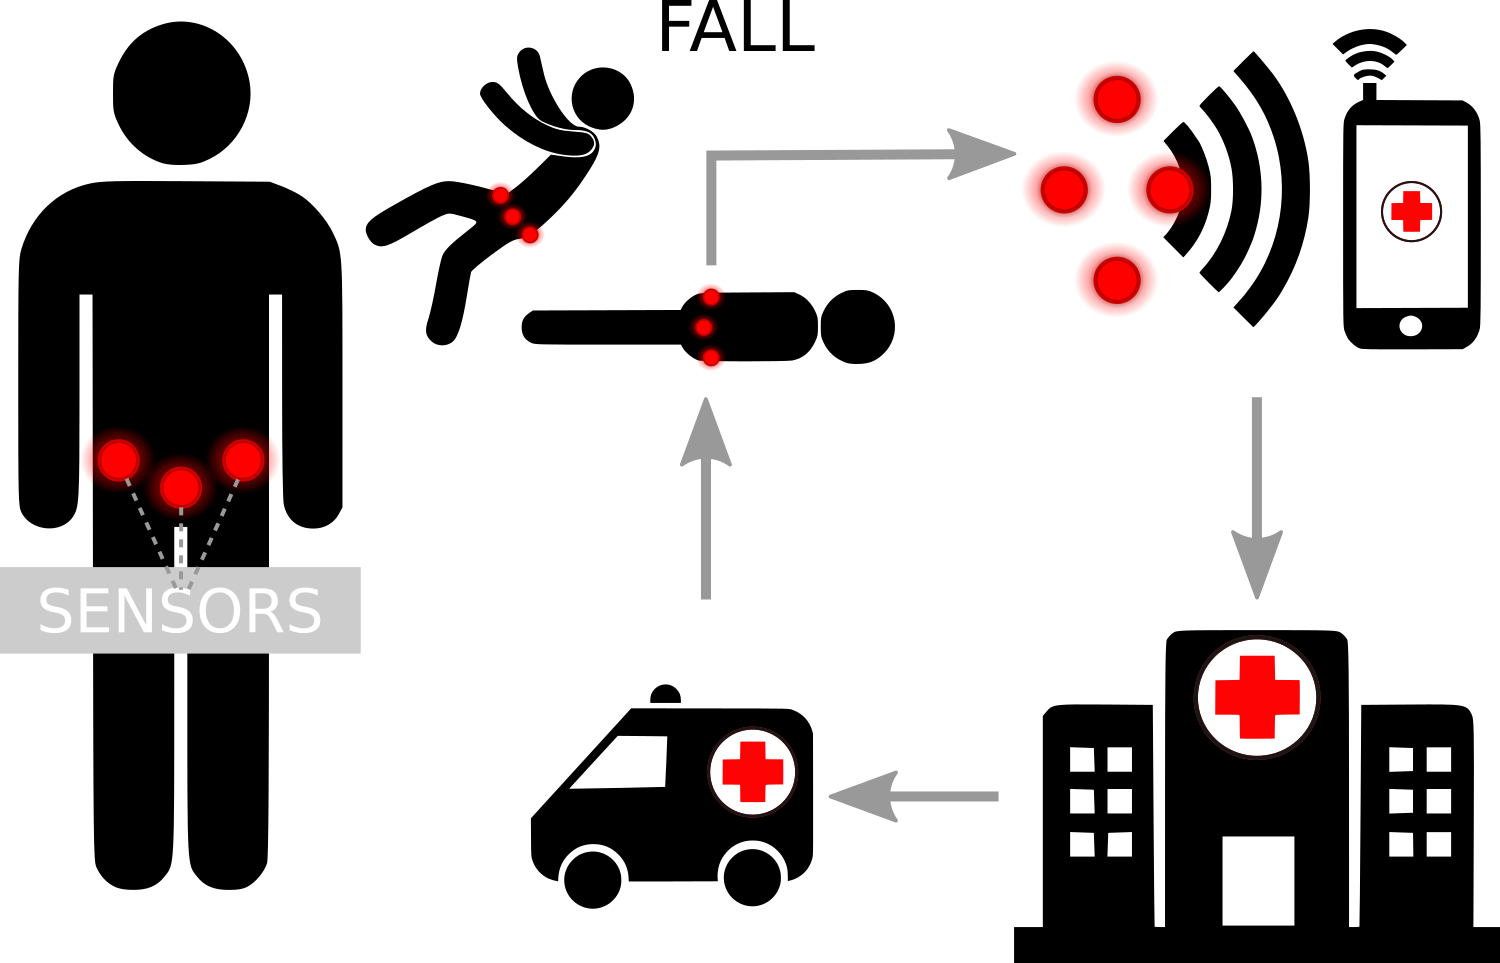
\includegraphics[scale=0.12]{img/Figure1}
  \caption[Escalation scheme]{Scheme fall simulation where a person has a wareable sensor network in form of a belt.~\cite{LaBlunda.2016,LaBlunda.2016b}}
  \label{fig:escalationscheme}
\end{figure}

The EPLs have been designed to address the main problems of 
IoT systems. In particular, EPLs are used to define critical situations in order to filter the 
information and to make correct decisions according to the obtained data. These critical 
situations are defined using event patterns and event rules. Among the existing EPLs, the 
EPL of EsperTech~\cite{Esper:2016} is used the most often. In our study, the critical situations are the falls,
so the obtained data from the mentioned prototype are used to define an EPL of EsperTech 
pattern to detect falls.

The first step of this prototype is to identify a fall from a fast movement, a sitting or laying 
down movement, but the final goal of the system is to predict the falls and act to prevent 
them. Given that to test this system is crucial, test events which simulate falls are necessary. In 
the literature different type of falls can be found, and it is necessary to identify all of them in 
order to tell them apart from a non-fall: in this study, two types of falls will be analysed. 

IoT-TEG~\cite{TesisGutierrez2017,Gutierrez2017} is a tool which automatically generates test events 
of many types. Thanks to the obtained data from the sensors we have checked that the measured 
parameter during a fall, the acceleration, has a specific behaviour. As a consequence, the test events 
must be generated according to its behaviour. This problem is solved with the new functionality that 
IoT-TEG includes which is introduced in this paper. %Moreover, the ongoing fall detection prototype will 
%be analysed and its improvements will be described; the new functionality of IoT-TEG can be adapted 
%according to the improvements of the fall detection prototype. 

In this study of falls as relevant situations, our main contributions are:

\begin{itemize}
\item \textbf{A study of the fall detection prototype evolution}: the system which is been used is
 continuously being improved. We describe the evolution of its architecture, how the data is analysed and 
 the detected problems.
 \item \textbf{An analysis of the major parameter in a fall}: while a person is falling, the acceleration 
 is the parameter that can measure the movement of the body. This parameter is analysed in order to know 
 its behaviour during two types of falls.
 \item \textbf{New definitions of two types of falls}: after the analysis of the acceleration during two 
 types of falls a new definition for each one has been done. The obtained data of the fall-detection 
 prototype is used to define EPL of EsperTech patterns to detect those types of falls. 
 \item \textbf{A new functionality of the IoT-TEG system} which allows to simulate the behaviour of 
 different event attributes in order to generate test events following a specific pattern. 
\end{itemize}

The rest of this paper is organised as follows. Section~\ref{sec:relatedwork}
describes not only the related work of event generators, but also the existing
solutions for fall-detection. Section~\ref{sec:background} provides the basic
knowledge of falls and EPLs. A brief introduction of IoT-TEG and its new functionality
appear in Section~\ref{iotteg}. The architecture of the fall detection system and the 
fall analysis are introduced in Section~\ref{sec:basicprototype}. Section~\ref{sec:improvedprototype}
describes the improvements on the prototype, a new fall type analysis,
a comparison of the obtained results and some detected problems. Finally, in Section~\ref{sec:conclusions}, 
we conclude our paper and make recommendations for future work.

\section{Related work}
\label{sec:relatedwork}

An overview about event generators reveals that the first event generators~\cite{dobbs2004houches,mangano2005tools}
were focused on extremely specific topics such as environmental conditions for the simulation of high energy 
physics events at particle colliders. Nowadays, we can find papers that address the same issues~\cite{Grzegorczyk}, but 
the technology surrounds us and the people and business need to control and monitor the things around them. 
The received information allows them to make decisions and to act according to it. This is the reason 
of the creation of the IoT platforms, which are the key for the development of scalable IoT applications and 
services that connect objects, systems and people to each other. However, not every IoT platform is a real IoT 
platform~\cite{iot-analytics:2015}; for instance, some event generators that are integrated in an enterprise 
software packages, which are increasingly allowing the integration of IoT devices, are often not advanced enough
to be classified as a full IoT platform. Examples are given in the following lines:

\begin{itemize}
 \item The Timing System~\cite{Finland:2016} provides a complete timing distribution system including timing signal 
 generation. Its event generator is responsible for creating timing events which are sent out as serialised event frames.
 \item The company Starcom~\cite{Starcom:2016} has developed an event generator to solve the problem of managing a huge 
 number of events. They state that their generator is capable of controlling the end event action, so the exact managers 
 requirements can be filtered. The tool is included in a kit distributed with their system.
 \item The WebLogic Integration Solutions~\cite{WebLogic:2016} allow the managing and monitoring of entities and 
 resources required for WebLogic Integration applications. This system contains an event generator module which allows the 
 creation and deployment of the event generators included as part of WebLogic Integration. The mentioned events 
 generators allow to define event types but they are not capable to simulate a specific behaviour with a set of 
 generated events. The relevant situations in IoT systems are a sequence of activities with a determined behaviour; 
 that is why IoT-TEG~\cite{TesisGutierrez2017,Gutierrez2017} includes this option.
\end{itemize}

Talking about fall-detection, there are several solutions that propose wearable sensors.
We are going to focus our attention on the approach proposed by Li et al.~\cite{Li2009}; their wearable fall-detection solutions,
which will be explained subsequently, was used for the development of our prototype. They introduce a fall-detection method based on a BAN that consists 
of two wearable sensor nodes. These two nodes comprise an accelerometer and gyroscope and are worn on the chest, node A, and thigh 
node B, (see Figure~\ref{fig:simulation}). The principle of this method differentiates between static postures and dynamic postures: 

\begin{itemize}
 \item Static postures: standing, sitting, laying and bending.
 \item Dynamic postures
 \begin{itemize}
  \item Activities of daily life: walking, walk on stairs, sit, jump, lay down and run.
  \item Fall-like motions: quick sit down upright and quick sit-down reclined.
  \item Flat surface falls: fall forward, fall backward, fall right and fall left.
  \item Inclined falls: fall on stairs.
 \end{itemize}
\end{itemize}

\begin{figure}[!ht]
  \centering
  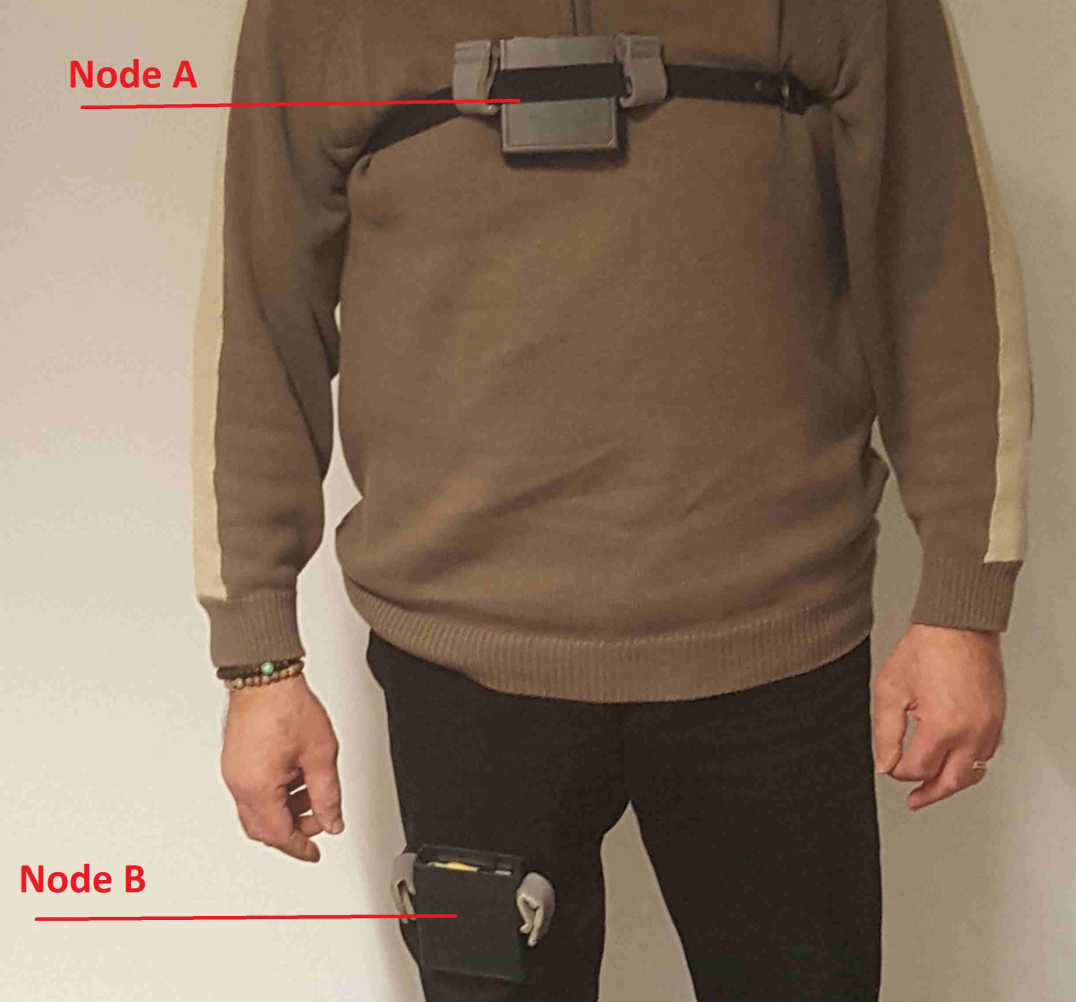
\includegraphics[scale=0.15]{img/BasePrototype.png}
  \caption[System architecture]{System architecture according to Li et al.~\cite{Li2009}}
  \label{fig:simulation}
\end{figure}

To decrease the computational effort of the microcontroller a three-phase algorithm was proposed, which is structured 
as follows:

\begin{enumerate}
 \item Phase activity analysis: check if person is in a static or dynamic position.
 \item Phase position analysis: if existing posture coincides with static posture, check whether the current position corresponds to laying.
 \item Phase state transition analysis: if in laying position, examine whether this transition was intentional or unintentional. The previous 5 
 seconds are used to analyse it. In the case that this position was unintentional, the system classifies it as a fall. 
\end{enumerate}

The weak point of this method is the differentiation between the activity \textit{jumping into bed} and the fall type \terxtit{falling against a wall with seated posture}.

\section{Background}
\label{sec:background}

\subsection{Fall analysis}
\label{subsec:analysis}

The approach used to detect falls is based on the basic idea proposed by~\cite{Gjoreski2014,Kozina}. A typical acceleration pattern during 
a fall-event is a decreasing acceleration close to 0g (free fall), followed by an increasing acceleration value (see Figure~\ref{fig:grafica}). In a stationary position, 
the acceleration measured is around 1g (9.81$m/s^{2}$) and during falling around 0g (0$m/s^{2}$). Upon the impact to the ground (fall-event), 
the maximum acceleration (peak-value) is reached for a short time period and it is greater than 1g. This pattern can be used to 
detect fall-events using the integrated accelerometer of the sensor nodes. Important to know is that the acceleration 
magnitude which is illustrated in the Formula~\ref{eq:acel} was used for the fall-detection:

\begin{equation}\label{eq:acel}
 \alpha = \sqrt{\alpha_{x}^{2} + \alpha_{y}^{2} + \alpha_{z}^{2}}
\end{equation}

\begin{figure}[!ht]
  \centering
  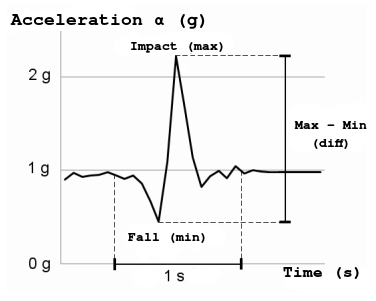
\includegraphics[scale=0.5]{img/FallGraph}
  \caption[Acceleration during impact]{Acceleration during impact~\cite{Kozina}.}
  \label{fig:grafica}
\end{figure}

Taking into consideration the depicted Figure~\ref{fig:grafica}, we can apply the following rule to evaluate the incoming acceleration data:

\begin{equation}\label{eq:caida}
 \alpha_{max} - \alpha_{min} > 1g
\end{equation}

in a 1 second window and $\alpha_{min}$ preceded $\alpha_{max}$; where $\alpha_{max}$ is the maximum acceleration value, 
$\alpha_{min}$ is the minimum acceleration value and $1g\approx9.81m/s^{2}$. Looking at the rule an event is categorised as a fall when the 
difference between $\alpha_{max}$ and $\alpha_{min}$ is greater than 1g and $\alpha_{min}$ is followed by $\alpha_{max}$. 
Important: this should happen within a time window of 1 second due to the fact, that a fall can occur in less than 1 second~\cite{Luder2009}.
To apply this rule we used the EPL of EsperTech~\cite{Esper:2016} in an IoT system which detects falls.

\subsection{Fall patterns with EPL of EsperTech}

Etzion and Niblett~\cite{Etz10} defined \textit{event processing agents} as software modules that process events. Such agents are specified using an 
EPL, and there are a number of styles of EPLs in use. The following styles are included: rule-oriented, imperatives and stream-oriented.

The EPL our work is based on is EPL of Esper~\cite{Esper:2016}, a stream-oriented language. The main reasons of its selection are: 
it is an extension of Structured Query Language (SQL), it can be embedded into Java applications and it is open source. 
% On the other hand, it is executed by Esper, a
% CEP engine which can process around 500.000 events per second on a workstation, and between 70.000 and 200.000 events per second on a laptop (according to 
% the company EsperTech).
 
% Unlike SQL that operates on tables, the EPL operates on a continuous stream of events. As a 
% result, a row from a table in SQL is analogous to an event present in an event stream. 
An EPL statement starts executing continuously during runtime. While the execution is taking place, EPL queries will be triggered if the application receives pre-defined or timer triggering events.
 
 \renewcommand{\lstlistingname}{Example}
 
 \begin{lstlisting}[basicstyle=\ttfamily\scriptsize,language=SQL,caption=EPL of EsperTech query example,label=EPLqueries]
select A as temp1, B as temp2 from 
  pattern [every temp1.temperature > 400 -> 
  temp2.temperature > 400]
 \end{lstlisting}
 
In the above example (see Example~\ref{EPLqueries}) of a ``nuclear
reactor control system'', its temperature gauges take a reading of the core temperature every second and send the data 
to a central monitoring system. The EPL of EsperTech query throws a warning if we have 2 consecutive 
temperatures above a certain threshold (400 degrees Celsius). This is a situation where a quick reaction to emerging patterns 
is needed in a stream of data events. A quick reaction is also needed in fall detection. 
% The pattern which 
% describes this situation will be shown in the corresponding section.
 
Because of the difficulties to simulate falls, IoT-TEG is used in
order to get the fall-test events automatically. 
IoT-TEG can be adapted or modified, if it is necessary, to generate any test events, even after the improvements 
in the fall-detection prototype.

\section{IoT test event generator}
\label{iotteg}

IoT-TEG~\cite{TesisGutierrez2017,Gutierrez2017} is a Java-based tool which takes an event 
type definition file and a desired output format %(JSON, CSV, and XML, the most common across 
%IoT platforms). 
IoT-TEG is made up of a \emph{validator} and an \emph{event generator} 
(Figure~\ref{fig:IoT-EGArquitecture}). The validator ensures the definition follows the rules set 
by IoT-TEG. The generator takes the definition and generates the indicated number of events according to it.

\begin{figure}[!ht]
  \centering
  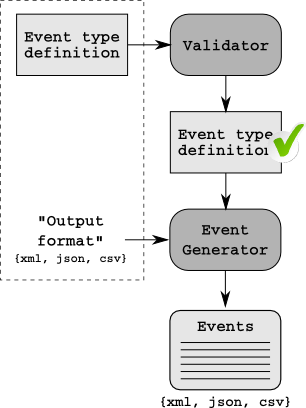
\includegraphics[scale=0.4]{./img/IoT-EGArquitecture}
  \caption[IoT-TEG Architecture]{IoT-TEG Architecture~\cite{TesisGutierrez2017,Gutierrez2017}.}
  \label{fig:IoT-EGArquitecture}
\end{figure}

Previous studies suggested there were no differences in testing effectiveness between using events
generated by IoT-TEG, or events recorded from various case studies~\cite{TesisGutierrez2017,Gutierrez2017}.
Moreover, thanks to its implementation, IoT-TEG can be used to do different types of tests: functional,
negative, integration, stress, etc; indeed an example of its usability can be found 
in~\cite{TesisGutierrez2017,gutierrez2018}, where IoT-TEG has been used to apply mutation 
testing~\cite{jia2011}. 

An event type is defined using XML language and its attributes have to be defined using the \texttt{\small{<field>}} element. 
A new property in IoT-TEG has been defined, the \texttt{\small{custom\_behaviour}}, which it is included in the 
\texttt{\small{<field>}} element to define the desired behaviour of any event attribute. In the \texttt{\small{custom\_behaviour}} 
property the path to the file that includes the behaviour of the event attribute has to be written. 

For the sake of clarity, Example~\ref{FallEvent} shows the complete fall event definition (FallEventType) that we are going
to use. The fall event type has one attribute, the acceleration, which follows an specific behavior depending on the type of fall.

\begin{lstlisting}[basicstyle=\ttfamily\scriptsize,language=XML,caption={Fall event type definition},label=FallEvent]
<?xml version="1.0" encoding="UTF-8"?>
<event name="FallEventType">
<block name="feeds" repeat="100">
 <field name="acceleration" quotes="false" type="Float" 
 custom_behaviour="/Path/To/Rule/File"></field>
</block>
</event>
\end{lstlisting}

In order to explain how the user has to define the desired behaviour of an event attribute, we are going
to use the behaviour of the acceleration during a fall (see Figure~\ref{fig:grafica}). In a XML file the 
number of simulations has to be indicated, the events involved in a simulation will be calculated according 
to the total number of events to generate and the desired simulations. For example, if the number of test 
events to generate is 100, this is indicated in the event type definition file (see Example~\ref{FallEvent}) as
\texttt{\small{repeat="100"}}, and if the number of desired simulations is 5, this is indicated as \texttt{\small{simulations="5"}}, 
in the behaviour rules definition file (see Example~\ref{FallRules}). So, the number of events 
involved to simulate the behaviour, a fall, is 20. 

Variables can be defined if they are needed in the behaviour rules definition file. They can be defined using 
the \texttt{\small{<variables>}} tags. To define them a name and a value 
have to be given to the variables. The value can be defined as a fixed value with the \texttt{\small{value}} 
property, or using a range with the \texttt{\small{min}} and \texttt{\small{max}} properties. For example, 
\texttt{\small{Base}} variable is used to define the acceleration of a person in a stationary position.
Some variables are involved in the value of another variables; this is indicated using the variable with an specific 
format \texttt{\small{\$(variable)}}. In addition, arithmetic operations can be done in the definition of the variable values. 

Once the variables are defined, the \texttt{\small{<rules>}} tags are used to define the acceleration behaviour in 
Figure~\ref{fig:grafica}. A \texttt{\small{weight}} must be assigned to each behaviour rule to calculate the number 
of events to generate for each one for each simulation.
Following the example and the assigned \texttt{\small{weight}} in Example~\ref{FallRules}, if 20 events simulate 
a fall $20 * 0,25 = 5$ events will be generated for the first rule, another 5 events for the second rule,
1 event for the third rule, and the remained events for the fourth rule. We have to assign zero to the weight
\texttt{\small{weight="0"}} to indicate how the remained events have to be generated. 

To define the rules, \texttt{\small{min}}, \texttt{\small{max}} and \texttt{\small{value}} properties can be used as well as the arithmetic 
operations and the references to another variables, see Example~\ref{FallRules}. Moreover, the \texttt{\small{sequence}} property can be used to obtain
values lower or higher than the one generated previously. The \texttt{\small{sequence}} property values are \texttt{\small{inc}}, 
to increase the value, or \texttt{\small{dec}}, to decrease the value; examples of their usage will be shown in the following
sections.

Thanks to the included properties and parameters in the IoT-TEG new functionality, the desired behaviour rules can
be defined. In the fall rules, the involved event attribute is the acceleration, and its behaviour during the 
fall is defined by four rules: the stationary position values, first and fourth rules, will be obtained from a range 
from 9.81-0.25 to 9.81+0.25, because depending on the person and the place the acceleration can be different; the fall, the second rule, 
is defined as a range between 0 and the fifth part of $1g$, and the impact value, the third rule, is from a range between $2gs$ and $6gs$.

\begin{lstlisting}[basicstyle=\ttfamily\scriptsize,language=XML,caption={Rules to define a fall},label=FallRules]
  <?xml version="1.0" encoding="UTF-8"?>
  <custom_conditions simulations="5">
  <variables>
   <variable name="Base" value="9.81"/>
  </variables>
  <rules>
   <rule weight="0.25" min="$(Base)-0.25" max="$(Base)+0.25"/>
   <rule weight="1" min="$(Base)*2" max="$(Base)*6"/>
   <rule weight="1" min="0.0" max="$(Base)/5"/>
   <rule weight="0" min="$(Base)-0.25" max="$(Base)+0.25"/>
  </rules>
  </custom_conditions>
\end{lstlisting}

\section{Prototype}
\label{sec:basicprototype}

\subsection{Architecture}
\label{sub:basicprototypearchitecture}

The system architecture is an important part to provide a precise and reliable fall-analysis. 
Additionally, the aspect of patient compliance should be taken into consideration, because the 
system should be developed not only from the developer point of view, but it should be accepted 
by the patients. An important requirement of the elderly is that the hardware design must 
facilitate the freedom of movement. Furthermore, the system has to guarantee a reliable 
functionality and redundancy to protect the wearable system against
a total system failure. J{\"a}ms{\"a} et al.~\cite{jamsa2014fall} state that the best
position of an accelerometer is near the waist.
With reference to these aspects a BAN in form of a belt was developed which 
includes a five sensor nodes which is based on ZigBee/IEEE 802.15.4\footnote{\url{http://www.zigbee.org/}}.

\begin{figure}[!ht]
  \centering
  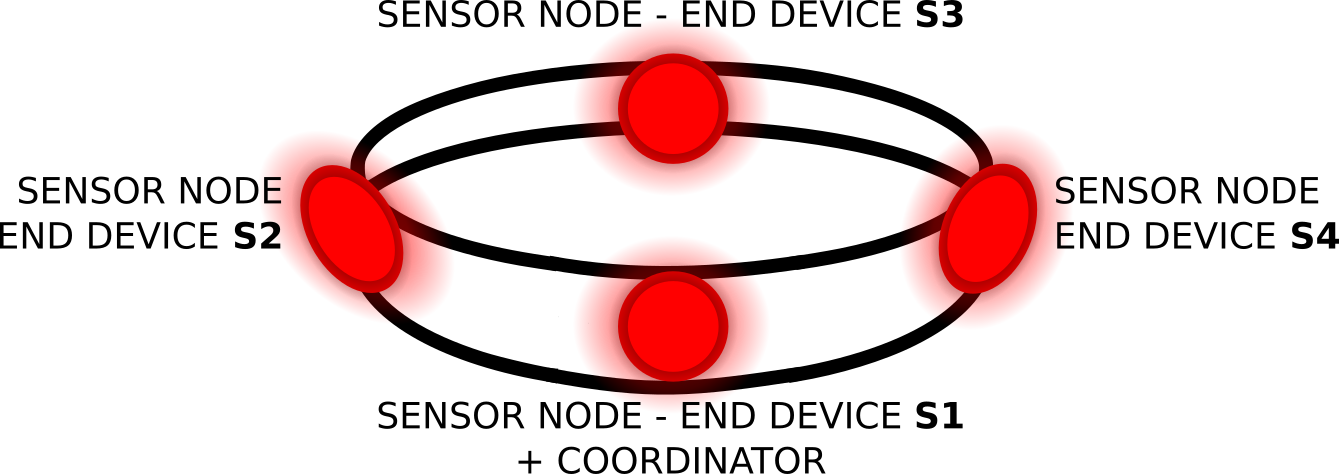
\includegraphics[scale=0.2]{./img/belt}
  \caption[Fall-detection belt]{Fall-detection belt~\cite{LaBlunda.2016,LaBlunda.2016b}}
  \label{fig:belt}
\end{figure}

Four of the sensor nodes are acting as end-devices (S1-S4) and the other node as a coordinator. 
The end-devices have attached an accelerometer and gyroscope which acquire continuously sensor 
data and is sent wirelessly to the coordinator using the ZigBee protocol. The data is sent in the following format:
 \begin{center}
  $|\alpha|, \omega_{x}, \omega_{y}, \omega_{z}$
 \end{center}
\begin{itemize}
  \item $|\alpha| \rightarrow$ This value
    represents the acceleration magnitude which is calculated by Formula (\ref{eq:acel}). 
    This value is a reference for impact detection. The unit measure is m/s$^2$.
  \item $\omega_{x}, \omega_{y}, \omega_{z} \rightarrow$ represent the angular velocity in X, Y and Z direction respectively. The unit measure is degree per second (dps).
\end{itemize}
The coordinator receives the incoming data and it has the function to evaluate the patient's status.

% The proposed positioning of sensors in the belt architecture was
% designed mainly for two reasons. The first reason  
% reflects the requirement of a safety critical system to which the
% fall-detection prototype belongs. The reliability  
% of the system must be ensured, in case one of the nodes fails. Using
% the architecture shown above (see Figure \ref{fig:belt}),  
% a mirroring of the opposing sensors is achieved with identical sensor values, only with different signs. 
% In case a node fails, the opposite value can be taken as a reference to detect a possible fall. The other reason for 
% applying the proposed architecture is that it significantly improves
% the accuracy of our system compared to earlier designs \cite{LuigiMasterThesis}. Taking into 
% consideration the following illustration (see Figure \ref{fig:axisreference}) the proposed belt architecture facilitates the recognition of several fall-types.
% 
% \begin{figure}[!ht]
%   \centering
%   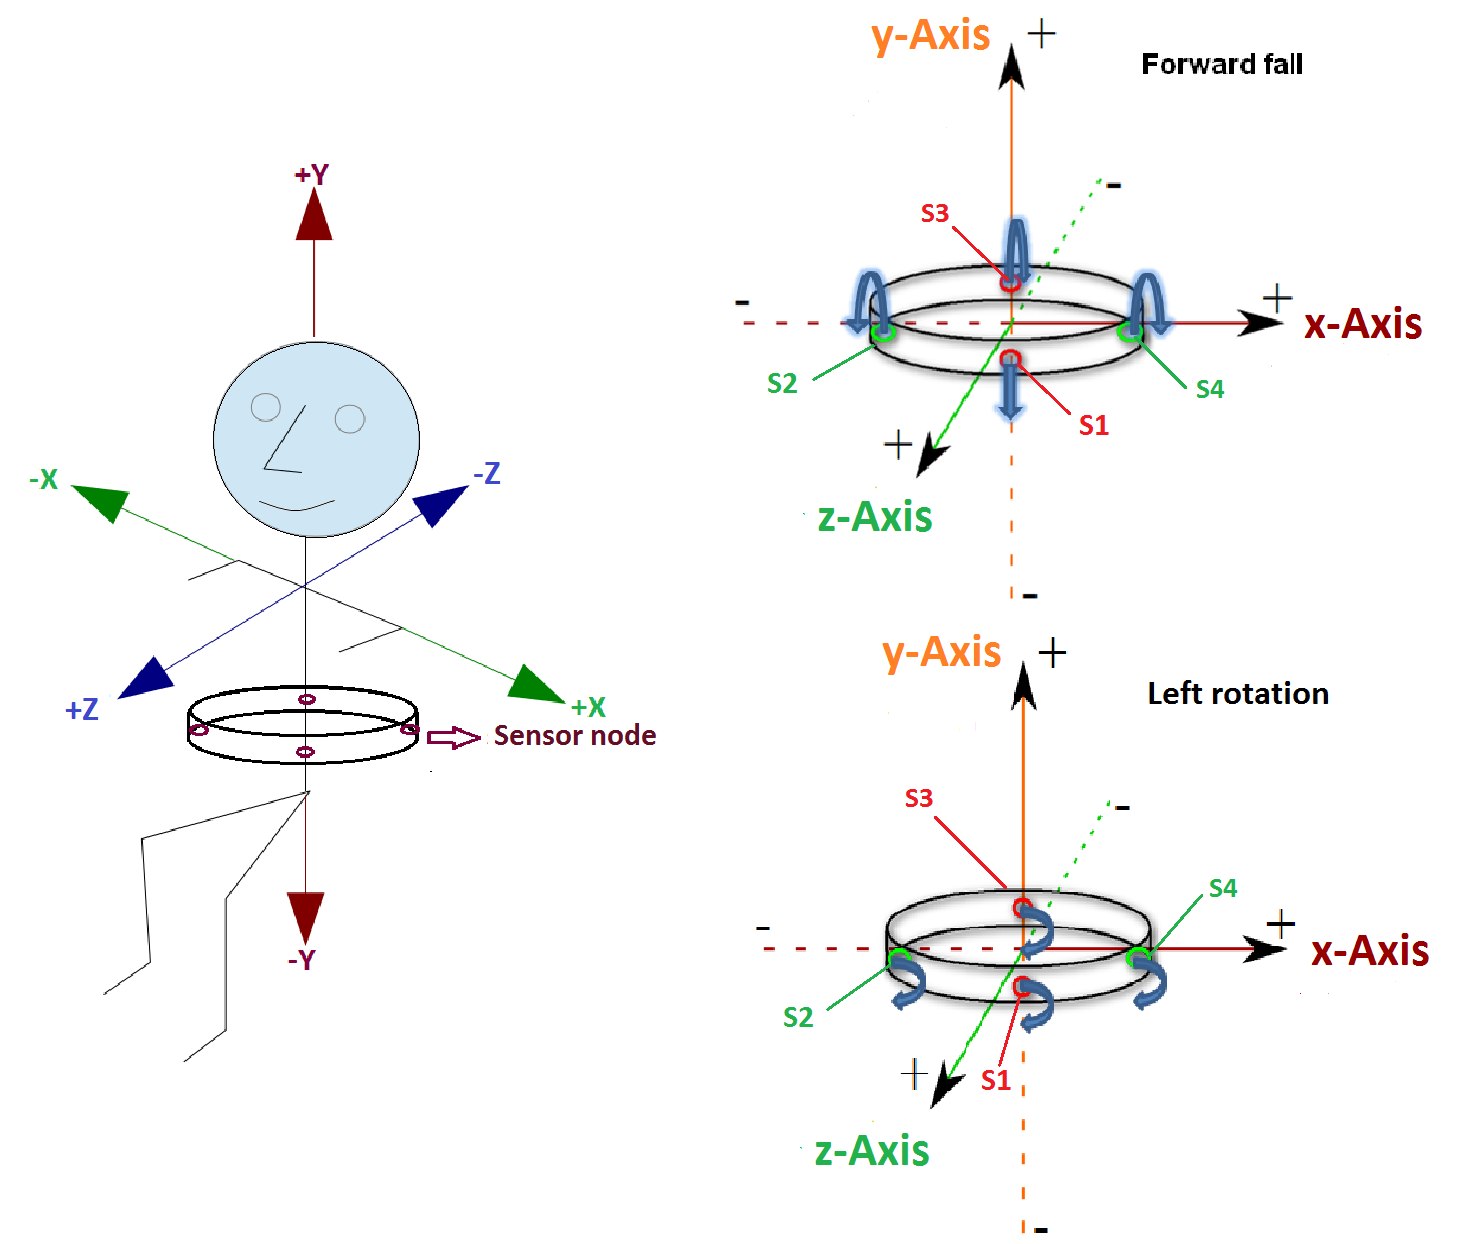
\includegraphics[scale=0.2]{./img/axis}
%   \caption[Three axis reference draft]{Three axis reference draft \cite{LaBlunda.2016b,LuigiMasterThesis}}
%   \label{fig:axisreference}
% \end{figure}
% 
% The special positioning of the nodes on the belt results in a more precise fall-characterisation. Considering 
% the event that a person does a left rotation and suffers a frontal impact to the ground (forward fall), 
% the gyroscope information (single values $\omega_{i}, i \in \{x,y,z\}$) could be used for the detection of rotation and the 
% acceleration magnitude $|\alpha|$ to detect the impact to the ground, see Equation (\ref{eq:acel}), Section~\ref{subsec:analysis}.

To test the system's accuracy different fall-types were reproduced with several test people. A 
test procedure based on Li et al.~\cite{Li2009} and Pannurat et al.~\cite{Pannurat2014} was developed which includes 
several motions and fall-types which are typical in nursing homes and hospitals.

Taking into account the architecture of the prototype and the rule to define a fall, see Formula (\ref{eq:acel}), 
the EPL of EsperTech pattern to define the fall situation is the one shown in the Example~\ref{FallPattern}.

\begin{lstlisting}[basicstyle=\ttfamily\scriptsize,language=SQL,caption=Fall pattern,label=FallPattern]
  select a1.accelS1, a2.accelS1, a1.accelS2, a2.accelS2 from 
   pattern [every(a1=BodyEvent(a1.accelS1 <= 9.81) -> 
   a2=BodyEvent(a2.accelS1 -a1.accelS1 >= 9.81 and 
   a1.PersonID = a2.PersonID) 
   where timer:within(1sec)) or every 
   (a1=BodyEvent(a1.accelS2 <= 9.81)
   -> a2=BodyEvent(a2.accelS2-a1.accelS2 >= 9.81
   and a1.PersonID = a2.PersonID) where timer:within(1sec))]
 \end{lstlisting}

The illustrated EPL query is based on the physical principle depicted in 
Figure \ref{fig:grafica}. Important to know is that for the EPL query two nodes 
were used (one frontal sensor node \& one lateral sensor node) to apply the 
fall-detection, but in the future this query will be extended to four sensor nodes. 
The four node architecture (see Figure \ref{fig:belt}) is currently only used 
for redundancy purposes. With the \textit{select} statement the event properties 
are selected to create a pattern for fall-detection. In the given example the
following event properties are selected:

\begin{itemize}
 \item \texttt{\small{a1.accelS1}}: starting acceleration value of node 1.
 \item \texttt{\small{a2.accelS1}}: subsequent acceleration value of node 1.
 \item \texttt{\small{a1.accelS2}}: starting acceleration value of node 2.
 \item \texttt{\small{a2.accelS2}}: subsequent acceleration value of node 2.
\end{itemize}

Taking into consideration the selected event properties the query checks if the 
starting acceleration of sensor node 1 is $<=$ 9.81 m/s$^2$ which means the person 
is in a stationary position in which the earth's gravity of 1g (9,81 m/$s^2$) acts 
on the body. Additionally, the subsequent acceleration of the first node checks if the subtraction of the subsequent acceleration and the first acceleration within a 
time window of 1 second is $>=$ 9.81 m/$s^2$ which means that the patient has 
suffered an impact to the ground. Using the \textit{OR} disjunction the second 
sensor node can be added and the statement is able to detect a fall in case one 
of the nodes matches the EPL query and the values of the acceleration correspond 
to the same person. 
 
\subsection{Fall simulation test events} 

Our goal is to study the acceleration behaviour during a fall in order to generate test events. The selected fall consists on rolling in the bed and fall (RBF)~\cite{Li2009,Pannurat2014}. In this study we have used a 
healthy subject, and we have recorded falls with all possible realism while also
trying to avoid risks. The person has been doing RBF type falls for a period of 2 minutes. The analysed 
data and videos can be found in~\cite{FallRepo}. In the following lines the steps to simulate 
the fall with the generated events are described, theses steps are very similar to the 
ones followed by~\cite{colladomachine,colladoTriaxal}:

\subsubsection*{1. Study of the values} Given that the sensor 1 is the one that suffers the
impact, its acceleration values are the first to be analysed. Figure~\ref{fig:Sensor1Sombras} 
shows the normalised acceleration data ($N(m/s^2)$) from sensor 1 while the person was falling. The normalised acceleration is
shown on the Y-axis, and the 
time in milliseconds (ms) on the X-axis.

While performing the data analysis, it has to be taken into account that the values suffer 
alterations because several factors: the person's movement, the person bouncing against something 
(floor, wall, etc), the collocation of the sensors to the original position after a fall, 
sensor pressure because of an impact or the person is laying over it, etc.

 \begin{figure}[!ht]
  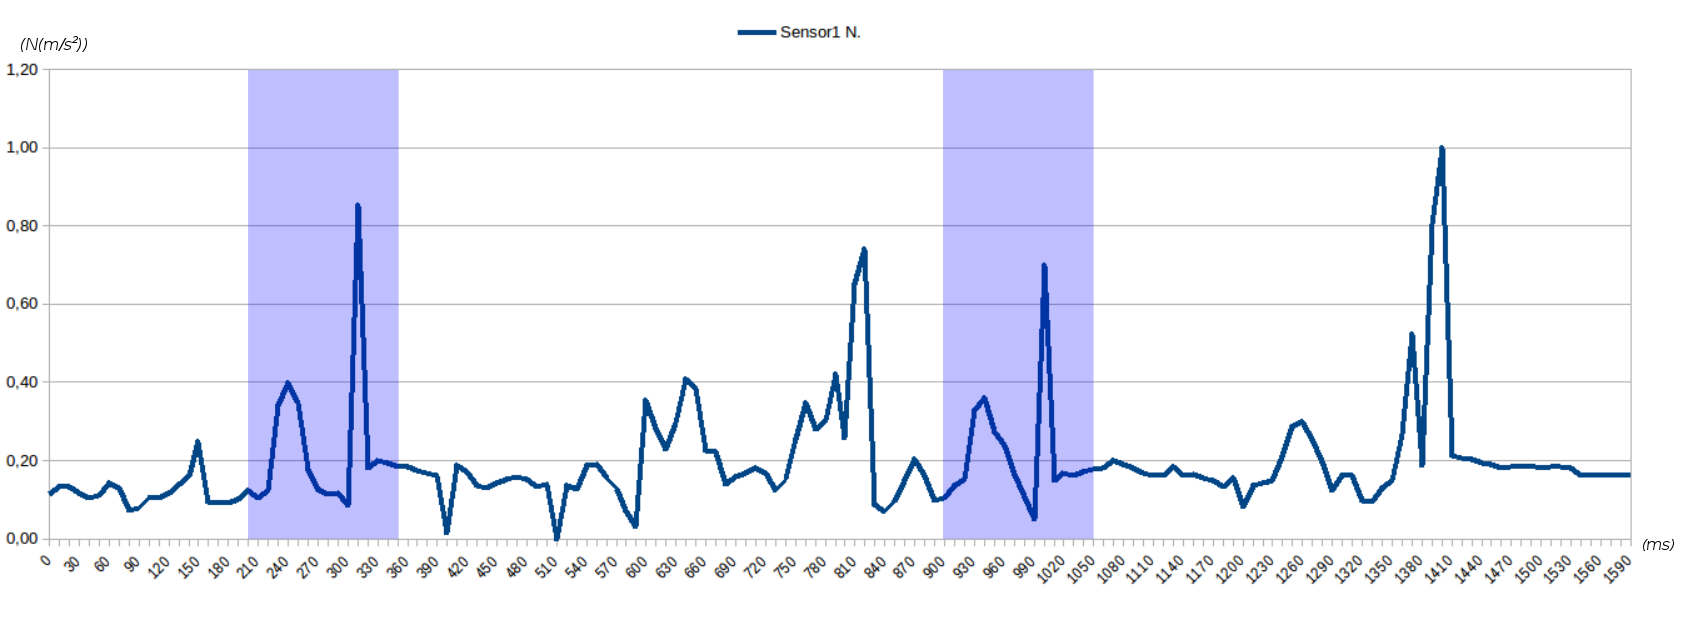
\includegraphics[scale=0.19]{img/Sensor1Sombras}
  \caption[Sensor 1 acceleration]{Sensor 1 acceleration.}
  \label{fig:Sensor1Sombras}
\end{figure}

\subsubsection*{2. Fall identification and analysis} After the previous study, the peaks of the acceleration are identified. 
These peaks, or maximum values, are when the sensor suffers the impact. We have considered a peak when the normalised acceleration is 
greater than 0,7 ($N(m/s^2) > 0,7$). Because of the mentioned noise, two ranges of the obtained 
values are extracted in order to analyse data properly. Please, see the highlighted parts in Figure~\ref{fig:Sensor1Sombras};
with respect to the X-axis $[210, 360]$ (Fall 1) and $[900, 1050]$ (Fall 2). The range of extracted values are a set of data that 
happen in less than a time window of 1 second, to meet the fact described in~\cite{Luder2009}. So as to compare both RBF falls
the acceleration values are normalised according to their impact value. The Table~\ref{tabla:RBF} 
shows the values to analyse where the impact value is highlighted with colour green.

\begin{table}[!ht]
 \centering
 \begin{tabular}{*{5}{r}}
   \centering
\begin{tabularx}{9cm}{@{}ccc|ccc@{}}
  \toprule
  \multicolumn{1}{p{0.65cm}}{\centering \textsc{Time} \\ ($s.ms$)} & \multicolumn{1}{p{0.65cm}}{\centering \textsc{Accel.} \\ ($m/s^2$)} & \multicolumn{1}{p{2cm}}{\centering \textsc{N. Accel.} \\ ($N(m/s^2)$)} & \multicolumn{1}{p{0.65cm}}{\centering \textsc{Time} \\ ($s.ms$)} & \multicolumn{1}{p{0.65cm}}{\centering \textsc{Accel.} \\ ($m/s^2$)}& \multicolumn{1}{p{2cm}}{\centering \textsc{N. Accel.} \\ ($N(m/s^2)$)} \\
  \midrule
0 & 6,29 & 0,02 & 0 & 5,98 & 0,08\\
10 & 7,57 & 0,05 & 10 & 6,31 & 0,08\\
20 & 20,7 & 0,33 & 20 & 8,2 & 0,13\\
30 & 24,07 & {\setlength{\fboxsep}{0pt}\colorbox{blue}{0,41}} & 30 & 9,21 & 0,16\\
40 & 21,01 & 0,34 & 40 & 19,92 & 0,43\\
50 & 10,81 & 0,12 & 50 & 21,8 & {\setlength{\fboxsep}{0pt}\colorbox{blue}{0,48}}\\
60 & 7,71 & 0,05 & 60 & 16,52 & 0,34\\
70 & 6,87 & 0,04 & 70 & 14,41 & 0,29\\
80 & 7,06 & 0,04 & 80 & 9,97 & 0,18\\
90 & 5,23 & {\setlength{\fboxsep}{0pt}\colorbox{bananayellow}{0,00}} & 90 & 6,54 & 0,09\\
100 & 51,58 & {\setlength{\fboxsep}{0pt}\colorbox{applegreen}{1,00}} & 100 & 3,01 & {\setlength{\fboxsep}{0pt}\colorbox{bananayellow}{0,00}}\\
110 & 11,01 & 0,12 & 110 & 42,34 & {\setlength{\fboxsep}{0pt}\colorbox{applegreen}{1,00}}\\
120 & 12,12 & 0,15 & 120 & 8,96 & 0,15\\
130 & 11,77 & 0,14 & 130 & 10,14 & 0,18\\
140 & 11,26 & 0,13 & 140 & 9,81 & 0,17\\
150 & 11,16 & 0,13 & 150 & 10,45 & 0,19\\
  \bottomrule
\end{tabularx}






 \end{tabular}
 \caption{RBF fall acceleration, fall (range) 1 and fall (range) 2}%
 \label{tabla:RBF}
\end{table}

The obtained data do not have a timestamp, so given that every 10 milliseconds the system sends the data, we have
divided the values according to this time. To compare the RBF falls the time in the Table~\ref{tabla:RBF} 
starts in 0 $ms$ and then increase in 10 $ms$, that is what it is shown in 
the first column of the Table. The second column shows the acceleration values ($m/s^2$) and the normalised acceleration values
are deployed in the third column ($N(m/s^2)$) according to the fall maximum value. In 
Figure~\ref{fig:Sensor1} a comparison of the normalised acceleration behaviour during the previous RBF falls is shown. 
This comparison shows a similar behaviour of the acceleration during the RBF falls.
Moreover, the acceleration in these two RBF falls follow the rule that define a fall, see Formula (\ref{eq:caida}).

\begin{figure}[!ht]
  \centering
  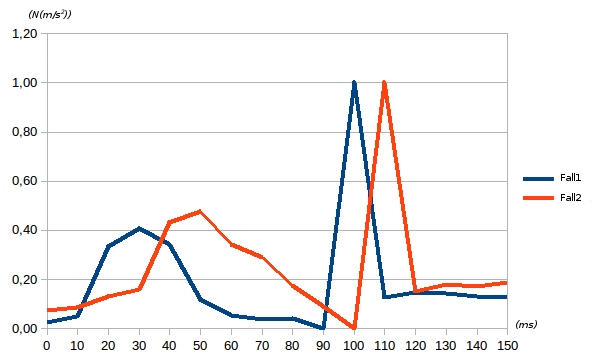
\includegraphics[scale=0.45]{img/Comparativa}
  \caption[Acceleration comparative]{Acceleration comparative.}
  \label{fig:Sensor1}
\end{figure}

The goal is to simulate this type of fall with events to test the IoT system, so we have to analyse the values of 
the acceleration before and after the impact. Taking into account that the maximum value of the acceleration is 
when the impact occurs ($\alpha_{max}$), the acceleration behaviour
during a RBF fall develops as follows:
\begin{enumerate}
 \item from a value less than the half of $\alpha_{max}$, the acceleration value increases to obtain a value in the range:
  \begin{center}
  $[\alpha_{max}/2 - 0.5, \alpha_{max}/2 + 0.5]$
  \end{center}
 The person is rolling on the bed.
 \item if the acceleration obtains a value in the previous range, its value decreases until the minimum value $\alpha_{min}$.
 The person is falling, a free fall.
 \item the acceleration value goes from the minimum value $\alpha_{min}$ to the maximum value $\alpha_{max}$. The person
 suffers the impact.
 \item the acceleration value is established with values around the half of $\alpha_{max}$. The person is laying on the floor. 
\end{enumerate}

The same analysis process has been done to the rest of sensors, and the behaviour of the acceleration of all of them 
follows the same pattern.

Taking into account the architecture of the prototype and the previous rules to define a RBF fall, the EPL of EsperTech
pattern to the define a RBF fall is the one shown in the Example~\ref{RBFpattern}.

%include mathscape to use use the option mathescape for your environment which gives you the ability to use the normal latex behavior of the $-signs
\begin{lstlisting}[basicstyle=\ttfamily\scriptsize,language=SQL, mathescape,caption=RBF pattern,label=RBFpattern]
select a1.accelS1, a2.accelS1, a3.accelS1, a4.accelS1 from 
pattern[every(a1 = BodyEvent(a1.accelS1 <= 9.81) -> 
a2 = BodyEvent(a2.accelS1 - a1.accelS1 >= 9.81) ->
a3 = BodyEvent(a3.accelS1 < 9.81) ->
a4 = BodyEvent(a4.accelS1 - a3.accelS1 >= 9.81 
and a2.accelS1 = a4.accelS1 / 2 $\pm$ 0.5) where 
timer:within(1sec))]
\end{lstlisting}

The displayed EPL query depicts a pattern which follows the mentioned rules and could be used to detect the rolling out of bed. 
Given that all the sensors are following the same pattern, one sensor node (S1) was used to create the query which makes it easier to understand it. 
%With the \textit{select} statement the event properties are selected to create a fall-detection pattern.
% In the given query the following event properties are selected:
% \begin{itemize}
%   \item \texttt{\small{a1.accelS1}}: starting acceleration value for stationary position (e.g. laying).
%   \item \texttt{\small{a1.accelS2}}: subsequent acceleration value for rolling event.
%   \item \texttt{\small{a1.accelS3}}: subsequent acceleration value for free fall event.
%   \item \texttt{\small{a1.accelS4}}: subsequent acceleration value for impact detection.
% \end{itemize}
% 
% Taking into consideration that the RBF fall is a complex event to detect, this event has been divided in the following phases: stationary phase (e.g. laying), rolling phase, free fall phase and impact phase.

The EPL query first checks if the starting acceleration \texttt{\small{a1.accelS1}} is $<=$ 9.81m/$s^2$ which means that the person is laying 
on the bed (stationary position). Additionally, the subsequent property is checked. If the difference between the successive 
acceleration value (\texttt{\small{a2.accelS1}}) and the previous one (\texttt{\small{a1.accelS1}}) is $>=$ 9.81 m/$s^2$ then the person has a transition to 
the rolling phase. If the person is falling after turning, the subsequent acceleration value should be $<$ 9.81 m/$s^2$ 
which means that the person is in the free fall phase. Additionally, if the difference between the current acceleration value 
(\texttt{\small{a4.accelS1}}) and the previous one (\texttt{\small{a3.accelS1}}) is
$>=$ 9.81 m/$s^2$, it is an indication for a fall. For a query to
recognise this event as a fall all these sequences should happen within a time window of 1 second.

\subsubsection*{3. To define the fall event} Once the fall acceleration behaviour has been observed, the next step is to define the 
fall event in order to generate test events with IoT-TEG~\cite{TesisGutierrez2017,Gutierrez2017}. Given that the involved event 
attribute in this fall is the acceleration, the Example~\ref{FallEvent} in Section~\ref{iotteg} can be used to define 
the fall event (FallEventType). The rules to define the behaviour of the acceleration in this type of fall is shown in 
Example~\ref{RBFFallRules}.

\begin{lstlisting}[basicstyle=\ttfamily\scriptsize,language=XML,caption={Rules to define a RBF fall},label=RBFFallRules]
  <?xml version="1.0" encoding="UTF-8"?>
  <custom_conditions simulations="5">
  <variables>
   <variable name="Impact" min="40.0" max="156.96"/>
   <variable name="Roll" min="$(Impact)/2-0.5" 
    max="$(Impact)/2+0.5"/>
   <variable name="Fall" min="0.0" max="$(Roll)/5"/>
  </variables>
  <rules>
   <rule weight="0.25" min="$(Roll)/4" max="$(Roll)" 
    sequence="inc"/>
   <rule weight="0.25" min="$(Roll)" max="$(Fall)" 
    sequence="dec"/>
   <rule weight="1" value="$(Impact)"/>
   <rule weight="0" min="$(Roll)/2-0.25" 
    max="$(Roll)/2+0.25"/>
  </rules>
  </custom_conditions>
\end{lstlisting}

To define the acceleration behaviour during a RBF fall three variables are defined: \texttt{\small{Roll}}, 
\texttt{\small{Fall}} and \texttt{\small{Impact}}. \texttt{\small{Impact}} will be the maximum value $\alpha_{max}$, 
\texttt{\small{Fall}} will be the minimum value $\alpha_{min}$ and the \texttt{\small{Roll}} variable is defined by a 
range where the acceleration value will be obtained according to the \texttt{\small{Impact}} value. In order to
obtain a low value, a range between 0 and the fifth part of \texttt{\small{Roll}} is assigned to the \texttt{\small{Fall}} 
variable.

In the RBF fall rules, the involved event attribute is the acceleration, and its behaviour during the 
fall is defined by four rules; in the first rule the acceleration value increases to a value close or equal to \texttt{\small{Roll}},
in the second rule the acceleration value decreases to a value close or equal to \texttt{\small{Fall}}, in the third rule the 
acceleration value is equal to \texttt{\small{Impact}}, it obtains the highest value and in the fourth rule the acceleration value
is established in a range which is lower than \texttt{\small{Roll}}.

It has to be emphasised that to obtain these rules for the definition
of the acceleration behaviour several tests
have been done. Once we obtained the desired results, test events were generated as they were necessary. The 
Figure~\ref{fig:IoTTEGRBFGeneratedEvents} shows the acceleration values of some of the generated RBF falls using
IoT-TEG and the new functionality. These generated events can be used to test the fall detection system.

\begin{figure}[!ht]
  \centering
  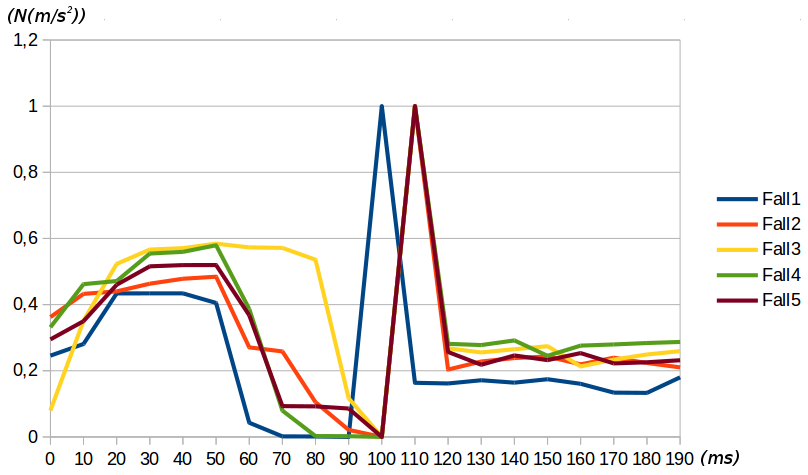
\includegraphics[scale=0.25]{img/IoTTEGRBFGeneratedEvents}
  \caption[IoT-TEG generated RBF falls]{IoT-TEG generated RBF falls.}
  \label{fig:IoTTEGRBFGeneratedEvents}
\end{figure}

\section{Improved prototype}
\label{sec:improvedprototype}

\subsection{Architecture}
\label{sub:improvedprototypearchitecture}

Taking into consideration the architecture of the prototype described in Section~\ref{sec:basicprototype} 
significant improvements were done. The improved hardware architecture is also 
based on four sensor nodes, but with the following significant innovations:

\begin{itemize}
 \item A new hardware platform which is based on Arduino Primo Core~\cite{Arduino2018}: 
 This microcontroller provides built-in sensors and a Bluetooth Low Energy (BLE) 
 interface for wireless data transmission. This satisfies the
 requiremnent of patient compliance
 which includes unrestricted movement.
 \item A different power supply mode is used for the improved prototype. Instead of 
 using the Lithium Polymer (LIPO) batteries, the Arduino Primo Core is supplied by a 
 coin cell. This is an important aspect due to the fact, that exposing the LIPO-batteries 
 to permanent shocks will damage them and drastically shorten their lifespan. 
 Additionally, with the usage of coin cells, we have reached a lifespan of 2 to 3 weeks 
 without exchanging the battery.
 \item The improved prototype is using BLE for wireless data transmission. Using BLE 
 brings the advantage to build up a communication infrastructure with the smartphone 
 to automatically inform the emergency services without any additional hardware.
 \item The dataset which is sent by the sensor nodes is composed as follows 
 and includes the values of $\alpha_{i}, i \in {x,y,z}$ in unit $m/s^{2}$:
 \begin{center}
  \texttt{\small{SensorID, X-Acceleration, Y-Acceleration, Z-Acceleration}}
 \end{center}
 Compared to the dataset format of the previous prototype, the sensor identification 
 number was added, and the significantly change is that only the single axis values of 
 the accelerometer are sent. Based on the individual axis values of the accelerometer, 
 the orientation of the person can also be determined. 
%  Assuming the person is in a standing 
%  position, the x-axis corresponds to 1G ($\pm$ 9.81m/$s^2$) and the other two axes would be 
%  approximately 0G. This indicates that the person is standing. As the person changes 
%  position, the gravitational acceleration will occur on one of the other axis. For that 
%  reason, in the improved prototype the single axis values were taken as orientation 
%  reference. To detect the impact the single values were used to calculate the acceleration 
%  magnitude based on Equation (\ref{eq:acel}), see Section~\ref{subsec:analysis}.
\end{itemize}

\subsection{Fall simulation test events}

The second fall to generate the test events consists on the impact of the person with 
a wall and falling on the knees and then on the chest: \textit{fall against wall} (FAW). 
In this study we have used two healthy subjects, and we have recorded falls with all 
possible realism while also trying to avoid risks. They have been doing fall-tests for a period 
of 2 minutes, the FAW fall type. The analysed data and videos can be found in ~\cite{FallRepo}.

In this analysis the same steps that the ones described in Section~\ref{sec:basicprototype} 
have been done:

\subsubsection*{1. Study of the values} Given that the sensor 1 is the one that suffers the 
impact, its acceleration values are the first to be
analysed. The acceleration values are normalised ($N(m/s^2)$) and the impacts of the falls,
peaks are detected ($N(m/s^2) > 0,7$). After applying the previous rule in all the fall data 
and taking into account the alterations because the mentioned factors, the impacts are detected.

\subsubsection*{2. Fall identification and analysis} Once the peaks are detected, a range of values, 
including the peaks, are selected in order to analyse data properly and to study the acceleration 
behaviour during FAW fall. The range of extracted values are a set of data that happen in less 
than a time window of 1 second, to meet the fall rule of~\cite{Luder2009} described in 
Formula (\ref{eq:caida}). The Table~\ref{tabla:FAW} shows the 
acceleration value during one FAW fall of person 1 and person 2. 

\begin{table}[!ht]
 \centering
 \begin{tabular}{*{5}{r}}
   \centering
\begin{tabularx}{9.5cm}{@{}ccc|ccc@{}}
  \toprule
  \multicolumn{1}{p{0.65cm}}{\centering \textsc{Time} \\ ($s.ms$)} & \multicolumn{1}{p{0.65cm}}{\centering \textsc{Accel.} \\ ($m/s^2$)} & \multicolumn{1}{p{2cm}}{\centering \textsc{N. Accel.} \\ ($N(m/s^2)$)} & \multicolumn{1}{p{0.65cm}}{\centering \textsc{Time} \\ ($s.ms$)} & \multicolumn{1}{p{0.65cm}}{\centering \textsc{Accel.} \\ ($m/s^2$)}& \multicolumn{1}{p{2cm}}{\centering \textsc{N. Accel.} \\ ($N(m/s^2)$)} \\
  \midrule
57.311 & 3,63 & 0,01 & 25.254 & 8,53 & 0,09 \\
57.359 & 3,43 & 0,00 & 25.303 & 10,79 & 0,19 \\
57.408 & 7,85 & 0,17 & 25.352 & 11,28 & 0,22 \\
57.506 & 10,99 & 0,30 & 25.401 & 13,83 & 0,34 \\
57.506 & 6,47 & 0,12 & 25.449 & 9,42 & 0,13 \\
57.554 & 4,61 & 0,05 & 25.503 & 8,63 & 0,09 \\
57.603 & 4,22 & 0,03 & 25.546 & 0,89 & 0,10 \\
57.651 & 22,86 & {\setlength{\fboxsep}{0pt}\colorbox{bananayellow}{0,77}} & 25.596 & 8,04 & 0,07 \\
57.700 & 28,84 & {\setlength{\fboxsep}{0pt}\colorbox{bananayellow}{1,00}} & 25.645 & 13,93 & 0,35 \\
57.749 & 21,78 & {\setlength{\fboxsep}{0pt}\colorbox{bananayellow}{0,72}} & 25.693 & 22,7 & {\setlength{\fboxsep}{0pt}\colorbox{bananayellow}{0,76}} \\
57.800 & 9,03 & 0,22 & 25.742 & 10,59 & 0,19 \\
57.846 & 10,79 & 0,29 & 25.791 & 8,63 & 0,09 \\
57.900 & 10,79 & 0,29 & 25.841 & 8,34 & 0,08 \\
57.944 & 9,32 & 0,23 & 25.888 & 6,67 & 0,00 \\
57.996 & 13,15 & 0,38 & 25.937 & 17,46 & 0,51 \\
58.042 & 20,99 & 0,69 & 25.986 & 27,76 & {\setlength{\fboxsep}{0pt}\colorbox{bananayellow}{1,00}} \\
58.186 & 28,25 & {\setlength{\fboxsep}{0pt}\colorbox{bananayellow}{0,98}} & 26.082 & 11,58 & 0,23 \\
58.188 & 27,47 & {\setlength{\fboxsep}{0pt}\colorbox{bananayellow}{0,95}} & 26.084 & 11,38 & 0,22 \\
58.240 & 10 & 0,26 & 26.134 & 10,5 & 0,18 \\
58.286 & 10,99 & 0,30 & 26.181 & 8,83 & 0,10 \\
58.334 & 11,67 & 0,33 & 26.230 & 12,75 & 0,29 \\
  \bottomrule
\end{tabularx}


 \end{tabular}
 \caption{FAW fall acceleration, person 1 and 2}%
 \label{tabla:FAW}
\end{table}

The first and fourth columns of the Table~\ref{tabla:FAW} represent
the seconds ($s$) and milliseconds 
($ms$) when the acceleration was measured. The second and fifth columns show the acceleration 
values  ($m/s^2$) and in the third and sixth columns are deployed the normalised acceleration values 
($N(m/s^2)$) according to the fall maximum value. In Figure~\ref{fig:FAWcomparison} a comparison 
of the normalised acceleration behaviour during the previous FAW falls of person 1 and person 2 is 
shown. These comparisons show a similar behaviour of the acceleration during the fall.

\begin{figure}[!ht]
  \centering
  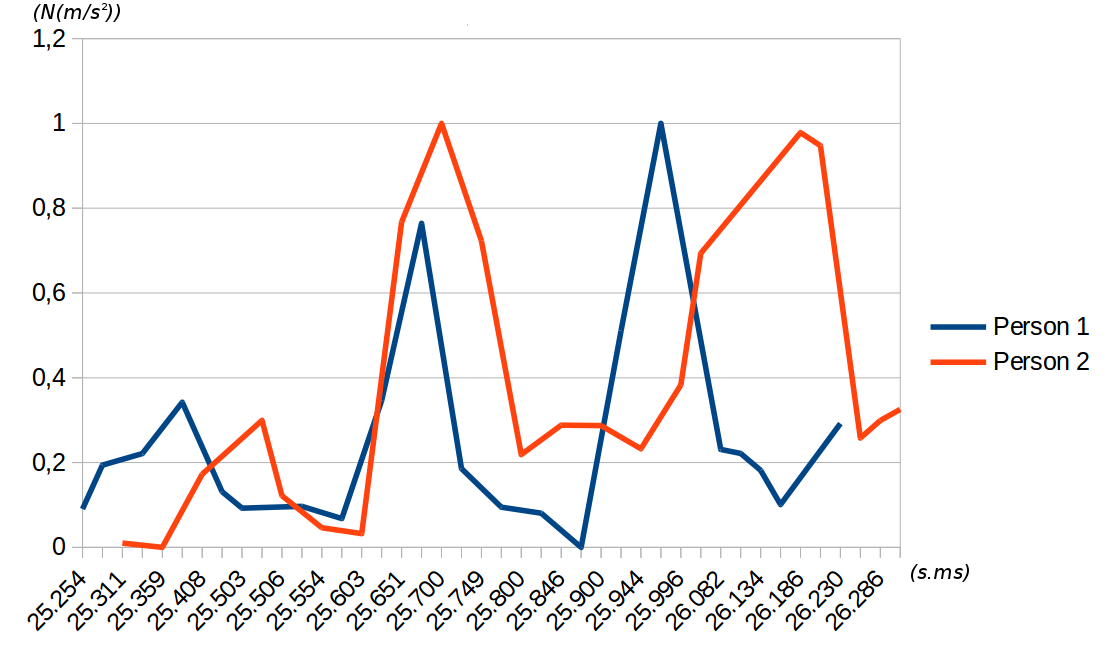
\includegraphics[scale=0.2]{img/TwoFallsComparative.png}
  \caption[Acceleration during FAW fall]{Acceleration comparison during FAW fall.}
  \label{fig:FAWcomparison}
\end{figure}

For the FAW, we have decided to define the acceleration behaviour with normalised values; so the 
normalised acceleration behaviour during the FAW consists on:
\begin{enumerate}
 \item the variation of its values while the person is walking. We have divided this rule in two rules:
 \begin{enumerate}
  \item The normalised acceleration values increase in a range [0, 0.35].
  \item The normalised acceleration values decrease in a range [0, 0.35].
 \end{enumerate}
 \item as a consequence of the impact of the person against a wall, the acceleration normalised value 
 has to be greater than 0.7.
 \item the normalised acceleration values decreases to a range [0, 0.35]. The values of the acceleration are 
 in the mentioned range depending on the size of the person; the larger person results in a longer range 
 and if the person retains a position prior to a fall thanks to the wall. Moreover, a subtle peak could 
 appear as a consequence of a rebound.
 \item a second impact happens when the person hit the ground, the acceleration normalised values has to 
 be greater than 0.7.
 \item finally, the person is laying on the ground and the normalised acceleration value decreases. The 
 values of the acceleration are between [0.10, 0.35] and no subtle peaks appear. 
\end{enumerate}

The same analysis process has been done to the rest of sensors, and the behaviour of the acceleration of all of 
them follows the same pattern.

Taking into account the architecture of the prototype and the previous rules to define a FAW fall, the EPL of EsperTech
pattern to the define a FAW fall is the one shown in the Example~\ref{FAWpattern}.

\begin{lstlisting}[basicstyle=\ttfamily\scriptsize,language=SQL, mathescape,caption=FAW pattern,label=FAWpattern]
select a1.accelS1, a2.accelS1, a3.accelS1, a4.accelS1, 
a5.accelS1 
from pattern[every(a1 = BodyEvent(a1.accelS1 >= 9.81) -> 
a2 = BodyEvent(a2.accelS1 < 9.81) ->
a3 = BodyEvent(a3.accelS1 - a2.accelS1 >= 9.81) ->
a4 = BodyEvent(a4.accelS1 < 9.81) ->
a5 = BodyEvent(a5.accelS1 - a4.accelS1 >= 9.81) 
where timer:within(1sec))]
\end{lstlisting}

% Considering the above EPL query, the following event properties are selected for the recognition of the FAW fall:

% \begin{itemize}
%   \item \texttt{\small{a1.accelS1}}: starting acceleration value for dynamic postures (e.g. walking).
%   \item \texttt{\small{a2.accelS1}}: successive acceleration value for free fall before wall impact.
%   \item \texttt{\small{a3.accelS1}}: subsequent acceleration value for wall impact.
%   \item \texttt{\small{a4.accelS1}}: successive acceleration value for free fall event.
%   \item \texttt{\small{a5.accelS1}}: subsequent acceleration value for impact to the ground.
% \end{itemize}

% This event has been divided in the following phases: dynamic phase (e.g. walking), free fall to wall phase, wall impact phase, free fall phase and impact phase.

The EPL query checks if the starting acceleration \texttt{\small{a1.accelS1}} is $>=$ 9.81 m/$s^2$ which means that the person is walking. 
The next acceleration value (\texttt{\small{a2.accelS1}}) is used to detect the free fall phase to the wall. If \texttt{\small{a2.accelS1}} 
is $<$ 9.81 m/$s^2$ it indicates that the person is falling against the fall. Additionally, if the difference between 
the current acceleration value (\texttt{\small{a3.accelS1}}) and the previous acceleration value (\texttt{\small{a2.accelS1}}) is $>=$ 9.81 m/$s^2$ 
it indicates the impact against a wall. After that, the person suffered the impact against a wall, the upcoming 
acceleration value (\texttt{\small{a4.accelS1}}) should be less than 9.81 m/$s^2$. This indicates that the person is falling to 
the ground. If the difference between the successive value (\texttt{\small{a5.accelS1}}) and the previous value (\texttt{\small{a4.accelS1}}) 
is $>=$ 9.81 m/$s^2$ it means that the person has suffered an impact to the ground. To classify this event as 
a FAW fall this pattern flow should happen within a time window of 1 second.

\subsubsection*{3. To define the fall event} Once the fall acceleration behaviour has been observed, the next step is to define the 
fall event in order to generate test events with IoT-TEG~\cite{TesisGutierrez2017,Gutierrez2017}. Given that the involved event 
attribute in this fall is the acceleration, the Example~\ref{FallEvent} can be used to define 
the fall event (FallEventType). The rules to define the behaviour of the acceleration in this type of fall is shown in 
Example~\ref{FAWFallRules}.

\begin{lstlisting}[basicstyle=\ttfamily\scriptsize,language=XML,caption={Rules to define a FAW fall},label=FAWFallRules]
  <?xml version="1.0" encoding="UTF-8"?>
  <custom_conditions simulations="5">
  <variables>
   <variable name="Base" value="9.81"/>
   <variable name="ImpactWall" min="$(Base)+$(Base)*0.7" 
    max="$(Base)*3"/>
   <variable name="Impact" min="$(Base)+$(Base)*0.7" 
    max="$(Base)*3"/>
  </variables>
  <rules>
   <rule weight="0.25" min="0" max="$(ImpactWall)*0.35" 
    sequence="inc"/>
   <rule weight="0.25" min="0" max="$(ImpactWall)*0.35" 
    sequence="dec"/>
   <rule weight="1" value="$(ImpactWall)"/>
   <rule weight="0.25" min="0" max="$(Impact)*0.35"/>
   <rule weight="1" value="$(Impact)"/>
   <rule weight="0" min="$(Base)+$(Base)*0.10"
    max="$(Impact)*0.35"/>
  </rules>
  </custom_conditions>
\end{lstlisting}

To define the acceleration behaviour during a FAW fall three variables are defined: \texttt{\small{Base}}, 
\texttt{\small{ImpactWall}} and \texttt{\small{Impact}}. Given that the acceleration behaviour during a FAW fall has
been according to the normalised values, the variables and rules have been defined according to 
that analysis. The acceleration value in a stationary position is a variable depending on the person, so 
we have considered the established value, $1g\approx9.81m/s^{2}$. That is the fixed value of the 
\texttt{\small{Base}} variable. To determine the values of the impacts, we have taken into account that the 
normalised value have to be $> 0,7$. So, to ensure that the impacts, \texttt{\small{ImpactWall}} and 
\texttt{\small{Impact}}, have a value meeting the mentioned condition the minimum value of the impact is  
\texttt{\small{Base}}$+$\texttt{\small{Base}}$*0,7$; and the maximum value of the
impacts is $3g\approx9,81*3=$\texttt{\small{Base}}$*3$.

Given that we have considered to define the FAW fall behaviour
rules according to the normalised values, the values to be generated depend on the maximum value. Due to this fact there are two values that can be the highest one, \texttt{\small{ImpactWall}} or \texttt{\small{Impact}}, the rules that depend on the maximum 
value contain the reference to the value, \texttt{\small{ImpactWall}} or \texttt{\small{Impact}}, according to the proximity
of the rule. For instance, the first and second FAW fall rules contain a reference to \texttt{\small{ImpactWall}}, the impact 
in the wall (third rule), which happens after the person is walking, something described in the first and the second rules.
The fourth and sixth rules contain a reference to \texttt{\small{Impact}}, the impact on the ground (fifth rule), which happens
after the person is falling and the person is laying on the floor, fourth and sixth rules.

It is important to highlight that to obtain these rules to define the behaviour of the normalised acceleration several tests
have been done. Once we obtained the desired results, test events were generated as they were necessary. The 
Figure~\ref{fig:IoTTEGFAWGeneratedEvents} shows the acceleration values of some of the generated FAW falls using
IoT-TEG and the new functionality.

\begin{figure}[!ht]
  \centering
  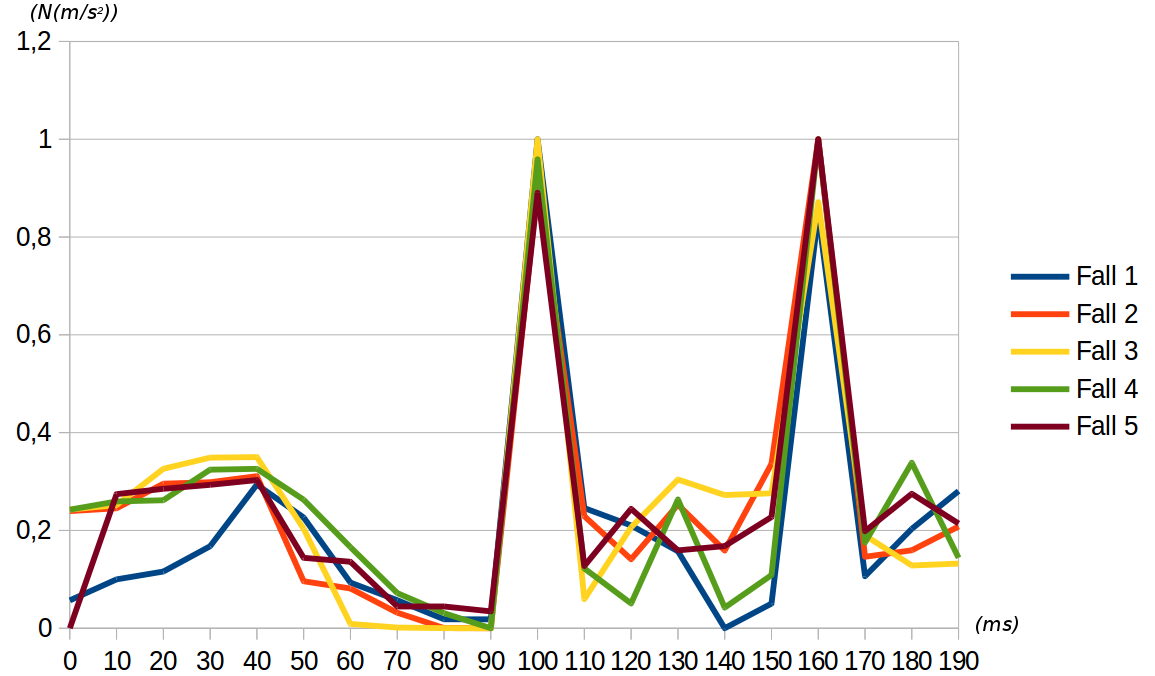
\includegraphics[scale=0.2]{img/IoTTEGFAWGeneratedEvents}
  \caption[IoT-TEG generated FAW falls]{IoT-TEG generated FAW falls.}
  \label{fig:IoTTEGFAWGeneratedEvents}
\end{figure}

The improvements in the new prototype are encouraging. They affect not only in the way of obtaining the data, but 
also in the format and their values. The impact values from one analysis to the other are quite different, 
this is because of several reasons described in Section~\ref{sub:detectedproblems}. The difference
of values was not a problem for IoT-TEG to define the behaviour rules and to generate the test events. That
means that the introduced functionality can be adapted to the analysed
behaviour. Moreover, it has to be emphasised that the application of the new functionality covers any event attribute which follows a behaviour;
so IoT-TEG is not limited.

\subsection{Detected problems}
\label{sub:detectedproblems}

After testing the current fall-detection prototype, some problems were 
found. Moreover, some considerations will be applied in future tests.

First of all, we are going to explain the problems related to the prototype: 

\begin{itemize}
 \item Synchronisation problem of the data acquisition with $n$ sensor nodes.
 \item Fall data from the beginning should always be discarded because
   the sensors start sending data at different times. The
   Table~\ref{tabla:Synchro} will be used to explain the problem. Let
   us say  
 that in ``fall 1'', there are more than 30 values that define the fall, and later in ``fall 3'', there are 
 12 values that define the fall. This is related to the synchronisation problem. So, in order to analyse the falls and compare the acceleration behaviour, it is 
 difficult to work with that information. A comparison of two FAW falls with the synchronisation problem is shown
 in Figure~\ref{fig:synchronisation1}; the sensor 1 acceleration values for the first FAW fall are coloured in blue and the
 sensor 1 acceleration values for the second FAW fall are coloured in red. The first fall is one fall from the beginning
 of the simulation, and the second one is from the middle of the simulation.
 
 \begin{table}[!ht]
 \centering
 \begin{tabular}{*{5}{r}}
   \centering
\begin{tabularx}{8cm}{@{}ccc|ccc@{}}
  \toprule
  \multicolumn{1}{p{0.65cm}}{\centering \textsc{Time} \\ ($s.ms$)}  &  \multicolumn{1}{p{0.65cm}}{\centering \textsc{Accel.} \\ ($m/s^2$)}  &  \multicolumn{1}{p{1.5cm}}{\centering \textsc{N. Accel.} \\ ($N(m/s^2)$)}  &  \multicolumn{1}{p{0.65cm}}{\centering \textsc{Time} \\ ($s.ms$)}  &  \multicolumn{1}{p{0.65cm}}{\centering \textsc{Accel.} \\ ($m/s^2$)} &  \multicolumn{1}{p{1.5cm}}{\centering \textsc{N. Accel.} \\ ($N(m/s^2)$)} \\
  \midrule
25.561 & 9,81 & 0,11 & 25.546 & 8,73 & 0,1 \\
25.561 & 9,81 & 0,11 & 25.596 & 8,04 & 0,07 \\
25.562 & 11,38 & 0,17 & 25.645 & 13,93 & 0,35 \\
25.564 & 11,38 & 0,17 & 25.693 & 22,76 & 0,76 \\
25.609 & 15,11 & 0,33 & 25.742 & 10,59 & 0,19 \\
25.610 & 15,11 & 0,33 & 25.791 & 8,63 & 0,09 \\
25.610 & 15,11 & 0,33 & 25.841 & 8,34 & 0,08 \\
25.611 & 15,11 & 0,33 & 25.888 & 6,67 & 0 \\
25.612 & 31,4 & 1 & 25.937 & 17,46 & 0,51 \\
25.612 & 23,84 & 0,69 & 25.986 & 27,76 & 1 \\
25.657 & 23,84 & 0,69 & 26.082 & 11,58 & 0,23 \\
25.657 & 23,84 & 0,69 & 26.084 & 11,38 & 0,22 \\
25.658 & 23,84 & 0,69 &  &  & \\
25.659 & 23,84 & 0,69 &  &  & \\
25.660 & 9,52 & 0,10 &  &  & \\
25.660 & 9,52 & 0,10 &  &  & \\
25.706 & 9,52 & 0,10 &  &  & \\
25.706 & 9,52 & 0,10 &  &  & \\
25.707 & 9,52 & 0,10 &  &  & \\
25.707 & 9,52 & 0,10 &  &  & \\
25.708 & 23,74 & 0,69 &  &  & \\
25.709 & 23,74 & 0,69 &  &  & \\
25.756 & 23,74 & 0,69 &  &  & \\
25.756 & 23,74 & 0,69 &  &  & \\
25.757 & 27,86 & 0,85 &  &  & \\
25.758 & 27,86 & 0,85 &  &  & \\
25.758 & 9,52 & 0,1 &  &  & \\
25.759 & 9,52 & 0,1 &  &  & \\
25.760 & 9,52 & 0,1 &  &  & \\
25.804 & 7,06 & 0 &  &  & \\
25.805 & 7,06 & 0 &  &  & \\
25.805 & 7,06 & 0 &  &  & \\
25.806 & 7,06 & 0 &  &  & \\
  \bottomrule
\end{tabularx}

 \end{tabular}
 \caption{Synchronisation problem, fall 1 and fall 2}%
 \label{tabla:Synchro}
 \end{table}
 
 \begin{figure}[!ht]
  \centering
  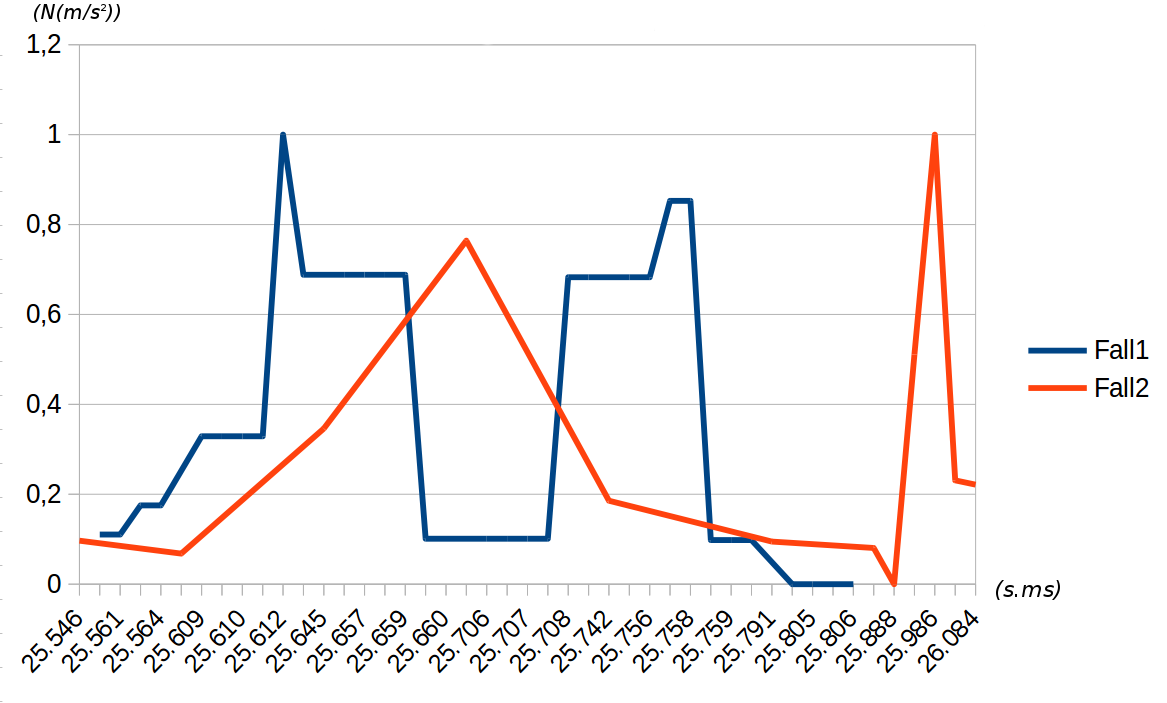
\includegraphics[scale=0.2]{img/synchronisation1.png}
  \caption[Comparison acceleration during two FAW falls]{Synchronisation problem; comparison of acceleration values during two FAW falls.}
  \label{fig:synchronisation1}
 \end{figure}
 
 The acceleration values show that in less than 250 milliseconds there are more than 30 values from ``fall 1'', and
 in more than 350 milliseconds there are 12 values from ``fall 2''. There is a lack of synchronisation not only in
 the amount of data, but also in the time.
 
 \item Some sensors transmit more data than the others, i.e. the sensors are not 
 sending the same amount of data, even sometimes there is no data. The four sensors were working while the FAW fall-simulation, but the obtained acceleration values were from three of them, one of the sensor did not transmit data 
 in one moment of the simulation, see Figure~\ref{fig:synchronisation2}.
 
 \begin{figure}[!ht]
  \centering
  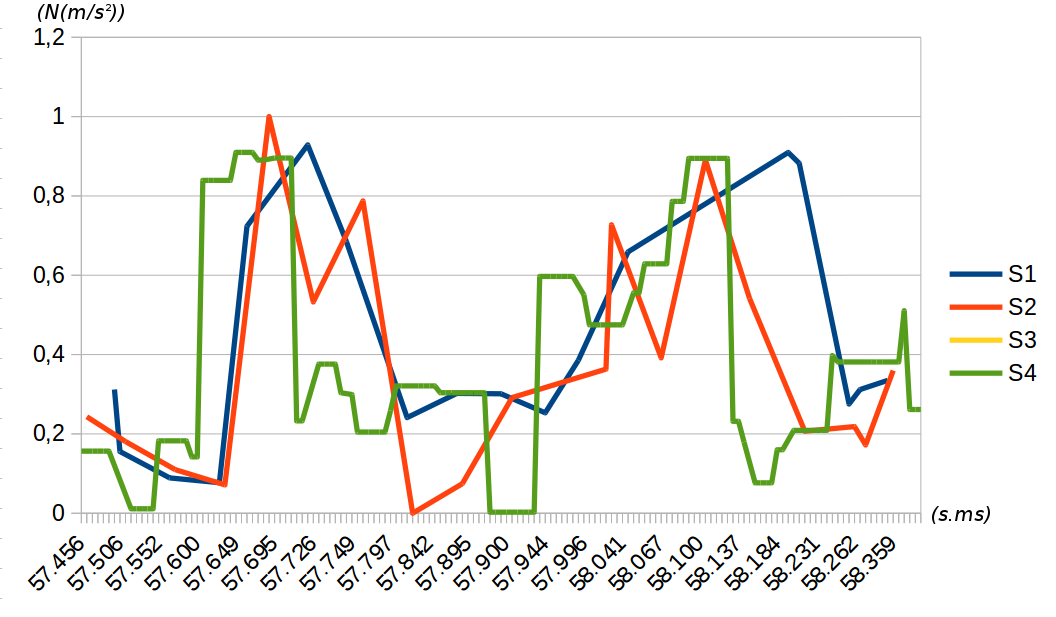
\includegraphics[scale=0.22]{img/synchronisation2.png}
  \caption[Comparison acceleration during two FAW falls]{Synchronisation problem; acceleration values from the four sensors during a FAW fall.}
  \label{fig:synchronisation2}
 \end{figure}
\end{itemize}

If we focus our attention to the hardware, the duration of the battery is also something to improve. Nowadays the 
duration of the battery is around 2 or 3 weeks, it depends on its use. If we want to use this IoT system with patients, 
specially with elderly people, or people that need special treatment, we have to increase the duration of the battery 
in order to change it as little as possible.

The analysis has revealed that while we were studying the acceleration data tests, some of its values could be misinterpreted.
This is because the test person that is falling for the simulation, stands up very fast. Given that we have been cautious
in our analysis and we have been checking not only the values but also the videos and matching them, we have detected
this issue. So, in our future tests, the test person should wait at least 2 seconds laying on the floor 
after the fall for a better fall simulation. In a real situation, if a
person falls and stands up this means that the person
is conscious and is able to move and call to the emergency services, if it is necessary. On the contrary, if the person
falls and does not stand up this means that maybe the person is unconscious or is not able to move and call the emergency
services. Therefore, waiting at least 2 seconds between falls in our test scenarios, it will help not only to understand 
better the behaviour of the acceleration values but also to do a better fall-simulation.

Comparing the measured values of the fall-events of the two 
prototypes, it can be determined that the measured impact values of the first prototype are considerably higher than 
those of the improved solution. This difference is caused by multiple reasons. The main reason is the different 
experimental set-up of the first prototype and the improved solution. The hardware design of the first prototype is 
bulky compared to the improved one. Due to the bulky construction the sensor nodes are more exposed to vibrations and 
shocks, which results in higher impact values. Additionally, the sensor nodes shifted during the fall. The result was 
that the test person repositioned the sensor nodes which leads to influence the impact value (acceleration magnitude). 
Taking this aspect into consideration, a smaller microcontroller
platform, which was described in \ref{sec:improvedprototype}, was used
to solve this problem. Despite the design differences in the two
prototypes,  
we are able to compare fall-types.

\section{Conclusions and Future Work}
\label{sec:conclusions}

We have ilustrated part of the process of the development of an IoT system to detect falls. This process
involves different types of testing, we have been using IoT-TEG~\cite{TesisGutierrez2017,Gutierrez2017}
to generate the test events in order to replicate the behaviour of the sample falls. The implemented functionality 
allows to generate events by defining rules which describe a desired behaviour. We can assign behaviour rules as many 
event attributes as the event type contains, and the values of each event attribute will follow the assigned behaviour.
The introduced functionality of IoT-TEG is able to adapt to the behaviour of the analysed event attribute, because
it was developed as a tool to generate test events for any system
which manages events and needs to be tested.

According to the falls, RBF and FAW, we have detected the necessity to define the
EPL query for each fall-type in the literature; this will
help to identify a fall from a no-fall. Moreover, it will be
interesting to add different types of sensors such as an air 
pressure sensor, and medical data such as ECG, in order to identify and characterise the falls.

The future work related to IoT-TEG~\cite{TesisGutierrez2017,Gutierrez2017} is to improve the tool in order to generate faithful 
test events which simulate the 
relevant situations that need to be filtered and, sometimes, are very difficult to imitate: adverse environment conditions, 
rise or fall in blood pressure, heart attack, falls... IoT-TEG is a
tool under development, so more functionalities will be added
to cover the test necessities. In order to improve IoT-TEG, more real events will be analysed which let us know 
the real situations and behaviour of the events.

% The introduced IoT-TEG functionality will be improved with a new property. This property will allow to generate values 
% which follow behaviour rules but depends from another event attribute value. IoT-TEG has the option
% to generate dependent values thanks to the \texttt{\small{dependence}} property. This property generates the event attribute value 
% according to a fixed value; so we will extend the tool with the option to define a dependence rule between event attributes. 

To generate test events, reliable data transmission of all four sensor nodes must be guaranteed. As described in 
the Section~\ref{sub:detectedproblems} the synchronisation problem can
lead to data loss during data transmission and  
thus influences the analysis of falls (see Table
\ref{tabla:Synchro}). For this reason, the use of a real-time system  
based microcontroller platform is planned, which facilitates the
synchronisation of the sensor nodes using a  
priority-controlled task scheduler. In addition, the battery lifespan
should be extended and the hardware design of the  
prototype should be as small as possible so that patients are not
restricted in their movements.

After studying the work of J{\"a}ms{\"a} et al.~\cite{jamsa2014fall}
we are going to include in our future work the analysis of 
the different postures after the fall. 

Fall-detection systems are safety critical. Therefore, new developments will include hazard analysis methods, e.g. STAMP/STPA, 
to satisfy safety standards, i.e. IEC61508, IEC60601, etc.

\section*{Acknowledgment}

Paper partially funded by The Ministry of Economy and Competitiveness (Spain) and the FEDER Fund, under the National Program for 
Research, Development and Innovation, Societal Challenges Oriented, Project DArDOS TIN2015-65845-C3-3-R, and the Program of
Development and Impulse of Research Activity of the University of Cadiz.


% An example of a floating figure using the graphicx package.
% Note that \label must occur AFTER (or within) \caption.
% For figures, \caption should occur after the \includegraphics.
% Note that IEEEtran v1.7 and later has special internal code that
% is designed to preserve the operation of \label within \caption
% even when the captionsoff option is in effect. However, because
% of issues like this, it may be the safest practice to put all your
% \label just after \caption rather than within \caption{}.
%
% Reminder: the "draftcls" or "draftclsnofoot", not "draft", class
% option should be used if it is desired that the figures are to be
% displayed while in draft mode.
%
%\begin{figure}[!t]
%\centering
%\includegraphics[width=2.5in]{myfigure}
% where an .eps filename suffix will be assumed under latex, 
% and a .pdf suffix will be assumed for pdflatex; or what has been declared
% via \DeclareGraphicsExtensions.
%\caption{Simulation results for the network.}
%\label{fig_sim}
%\end{figure}

% Note that the IEEE typically puts floats only at the top, even when this
% results in a large percentage of a column being occupied by floats.


% An example of a double column floating figure using two subfigures.
% (The subfig.sty package must be loaded for this to work.)
% The subfigure \label commands are set within each subfloat command,
% and the \label for the overall figure must come after \caption.
% \hfil is used as a separator to get equal spacing.
% Watch out that the combined width of all the subfigures on a 
% line do not exceed the text width or a line break will occur.
%
%\begin{figure*}[!t]
%\centering
%\subfloat[Case I]{\includegraphics[width=2.5in]{box}%
%\label{fig_first_case}}
%\hfil
%\subfloat[Case II]{\includegraphics[width=2.5in]{box}%
%\label{fig_second_case}}
%\caption{Simulation results for the network.}
%\label{fig_sim}
%\end{figure*}
%
% Note that often IEEE papers with subfigures do not employ subfigure
% captions (using the optional argument to \subfloat[]), but instead will
% reference/describe all of them (a), (b), etc., within the main caption.
% Be aware that for subfig.sty to generate the (a), (b), etc., subfigure
% labels, the optional argument to \subfloat must be present. If a
% subcaption is not desired, just leave its contents blank,
% e.g., \subfloat[].


% An example of a floating table. Note that, for IEEE style tables, the
% \caption command should come BEFORE the table and, given that table
% captions serve much like titles, are usually capitalized except for words
% such as a, an, and, as, at, but, by, for, in, nor, of, on, or, the, to
% and up, which are usually not capitalized unless they are the first or
% last word of the caption. Table text will default to \footnotesize as
% the IEEE normally uses this smaller font for tables.
% The \label must come after \caption as always.
%
%\begin{table}[!t]
%% increase table row spacing, adjust to taste
%\renewcommand{\arraystretch}{1.3}
% if using array.sty, it might be a good idea to tweak the value of
% \extrarowheight as needed to properly center the text within the cells
%\caption{An Example of a Table}
%\label{table_example}
%\centering
%% Some packages, such as MDW tools, offer better commands for making tables
%% than the plain LaTeX2e tabular which is used here.
%\begin{tabular}{|c||c|}
%\hline
%One & Two\\
%\hline
%Three & Four\\
%\hline
%\end{tabular}
%\end{table}


% Note that the IEEE does not put floats in the very first column
% - or typically anywhere on the first page for that matter. Also,
% in-text middle ("here") positioning is typically not used, but it
% is allowed and encouraged for Computer Society conferences (but
% not Computer Society journals). Most IEEE journals/conferences use
% top floats exclusively. 
% Note that, LaTeX2e, unlike IEEE journals/conferences, places
% footnotes above bottom floats. This can be corrected via the
% \fnbelowfloat command of the stfloats package.


% trigger a \newpage just before the given reference
% number - used to balance the columns on the last page
% adjust value as needed - may need to be readjusted if
% the document is modified later
%\IEEEtriggeratref{8}
% The "triggered" command can be changed if desired:
%\IEEEtriggercmd{\enlargethispage{-5in}}

% references section

% can use a bibliography generated by BibTeX as a .bbl file
% BibTeX documentation can be easily obtained at:
% http://mirror.ctan.org/biblio/bibtex/contrib/doc/
% The IEEEtran BibTeX style support page is at:
% http://www.michaelshell.org/tex/ieeetran/bibtex/
\bibliographystyle{IEEEtran}
% argument is your BibTeX string definitions and bibliography database(s)
%\bibliography{IEEEabrv,../bib/paper}
%
% <OR> manually copy in the resultant .bbl file
% set second argument of \begin to the number of references
% (used to reserve space for the reference number labels box)
% \begin{thebibliography}{1}
% 
% \bibitem{IEEEhowto:kopka}
% H.~Kopka and P.~W. Daly, \emph{A Guide to \LaTeX}, 3rd~ed.\hskip 1em plus
%   0.5em minus 0.4em\relax Harlow, England: Addison-Wesley, 1999.
% 
% \end{thebibliography}

\bibliography{references}


% that's all folks
\end{document}


